%=================================================================
\documentclass[Universe,article,submit,moreauthors,pdftex]{Definitions/mdpi} 
%=================================================================
\firstpage{1} 
\makeatletter 
\setcounter{page}{\@firstpage} 
\makeatother
\pubvolume{xx}
\issuenum{1}
\articlenumber{5}
\pubyear{2020}
\copyrightyear{2020}
%\externaleditor{Academic Editor: Roman Pasechnik}

%\preto{\abstractkeywords}{\nolinenumbers} %>>>>nolinenumbers<<<
%\history{Received: 10 September 2020; Accepted: date; Published: date}
%\updates{yes} % If there is an update available, un-comment this line

%% MDPI internal command: uncomment if new journal that already uses continuous page numbers 
%\continuouspages{yes}

%------------------------------------------------------------------
% The following line should be uncommented if the LaTeX file is uploaded to arXiv.org
\pdfoutput=1

%=================================================================
% Add packages and commands here. The following packages are loaded in our class file: fontenc, inputenc, calc, indentfirst, fancyhdr, graphicx,epstopdf, lastpage, ifthen, lineno, float, amsmath, setspace, enumitem, mathpazo, booktabs, titlesec, etoolbox, tabto, xcolor, soul, multirow, microtype, tikz, totcount, amsthm, hyphenat, natbib, hyperref, footmisc, url, geometry, newfloat, caption
\usepackage{xcolor}
\usepackage{graphicx}
\newcommand*{\req}[1]{Eq.~{\eqref{#1}}}
\newcommand*{\rf}[1]{Fig.~{\ref{#1}}}
\newcommand*{\rsec}[1]{Sect.\,{\ref{#1}}}
\newcommand*{\bb}{\boldsymbol}
\newcommand*{\xred}{\color{red}}
\newcommand*{\xblue}{\color{blue}}
\newcommand*{\xgreen}{\color{green}}

%=================================================================
%% Please use the following mathematics environments: Theorem, Lemma, Corollary, Proposition, Characterization, Property, Problem, Example, ExamplesandDefinitions, Hypothesis, Remark, Definition, Notation, Assumption
%% For proofs, please use the proof environment (the amsthm package is loaded by the MDPI class).

%=================================================================
% Full title of the paper (Capitalized)
\Title{\uppercase{Electron Positron Magnetization in the Early Universe}}

% Author Orcid ID: enter ID or remove command
\newcommand{\orcidauthorA}{0000-0001-8217-1484} % Add \orcidA{} behind the author's name
\newcommand{\orcidauthorB}{0000-0001-5038-8427} % Add \orcidB{} behind the author's name
\newcommand{\orcidauthorC}{0000-0001-5474-2649} % Add \orcidC{} behind the author's name
 
% Authors, for the paper (add full first names)
\Author{Johann Rafelski\orcidA{}, Cheng Tao Yang\orcidB{}, Andrew Steinmetz\orcidC{}, and Jeremiah Birrell}
% Authors, for metadata in PDF
\AuthorNames{Johann Rafelski, Cheng Tao Yang, Andrew Steinmetz, and Jeremiah Birrell}

% Affiliations / Addresses (Add [1] after \address if there is only one affiliation.)
\address[1]{%
Department of Physics, The University of Arizona, Tucson, Arizona 85721, USA} 

% Contact information of the corresponding author
\corres{Correspondence: JohannR@arizona.edu
%; %Tel.: (optional; include country code; if there are multiple corresponding authors, add author initials) +xx-xxxx-xxx-xxxx (F.L.)
}

% Current address and/or shared authorship
%\firstnote{Current address: Affiliation 3} 
%\secondnote{These authors contributed equally to this work.}
% The commands \thirdnote{} till \eighthnote{} are available for further notes

%\simplesumm{} % Simple summary

%\conference{} % An extended version of a conference paper

% Abstract (Do not insert blank lines, i.e. \\) 

\abstract{We will write abstract here}
%
\keyword{Magnetization; Electron-Positron plasma; Cosmology.}
%%%%%%%%%%%%%%%%%%%%%%%%%%%%%%%%%%%%%%%
\begin{document}
%%%%%%%%%%%%%%%%%%%%%%%%%%%%%%%%%%%%%%% 
\section{Introduction}
\noindent The electron-positron epoch of the early universe was home to several significant events which have greatly shaped our contemporary universe including neutrino decoupling, Big Bang Nucleosynthesis (BBN), the annihilation of most electrons and positrons partially re-ionizing the universe, as well as setting the stage for the eventual recombination period which would generate the cosmic microwave background (CMB). Therefore, correctly describing the dynamics of this $e^{\pm}$ plasma is of interest when considering modern cosmic mysteries such as the origin of extra-galactic magnetic fields (EGMF). While most approaches tackle magnetized plasmas from the perspective of magneto-hydrodynamics (MHD), a primarily classical or semi-classical approach, our perspective is to demonstrate that fundamental quantum statistical analysis can lead to further insights on the behavior of magnetized plasmas.
%%%%%%%%%%%%%%%%%%%%%%%%%%%%%%%%%%%%%%%
\begin{figure} 
  \centerline{\hspace*{0.4cm}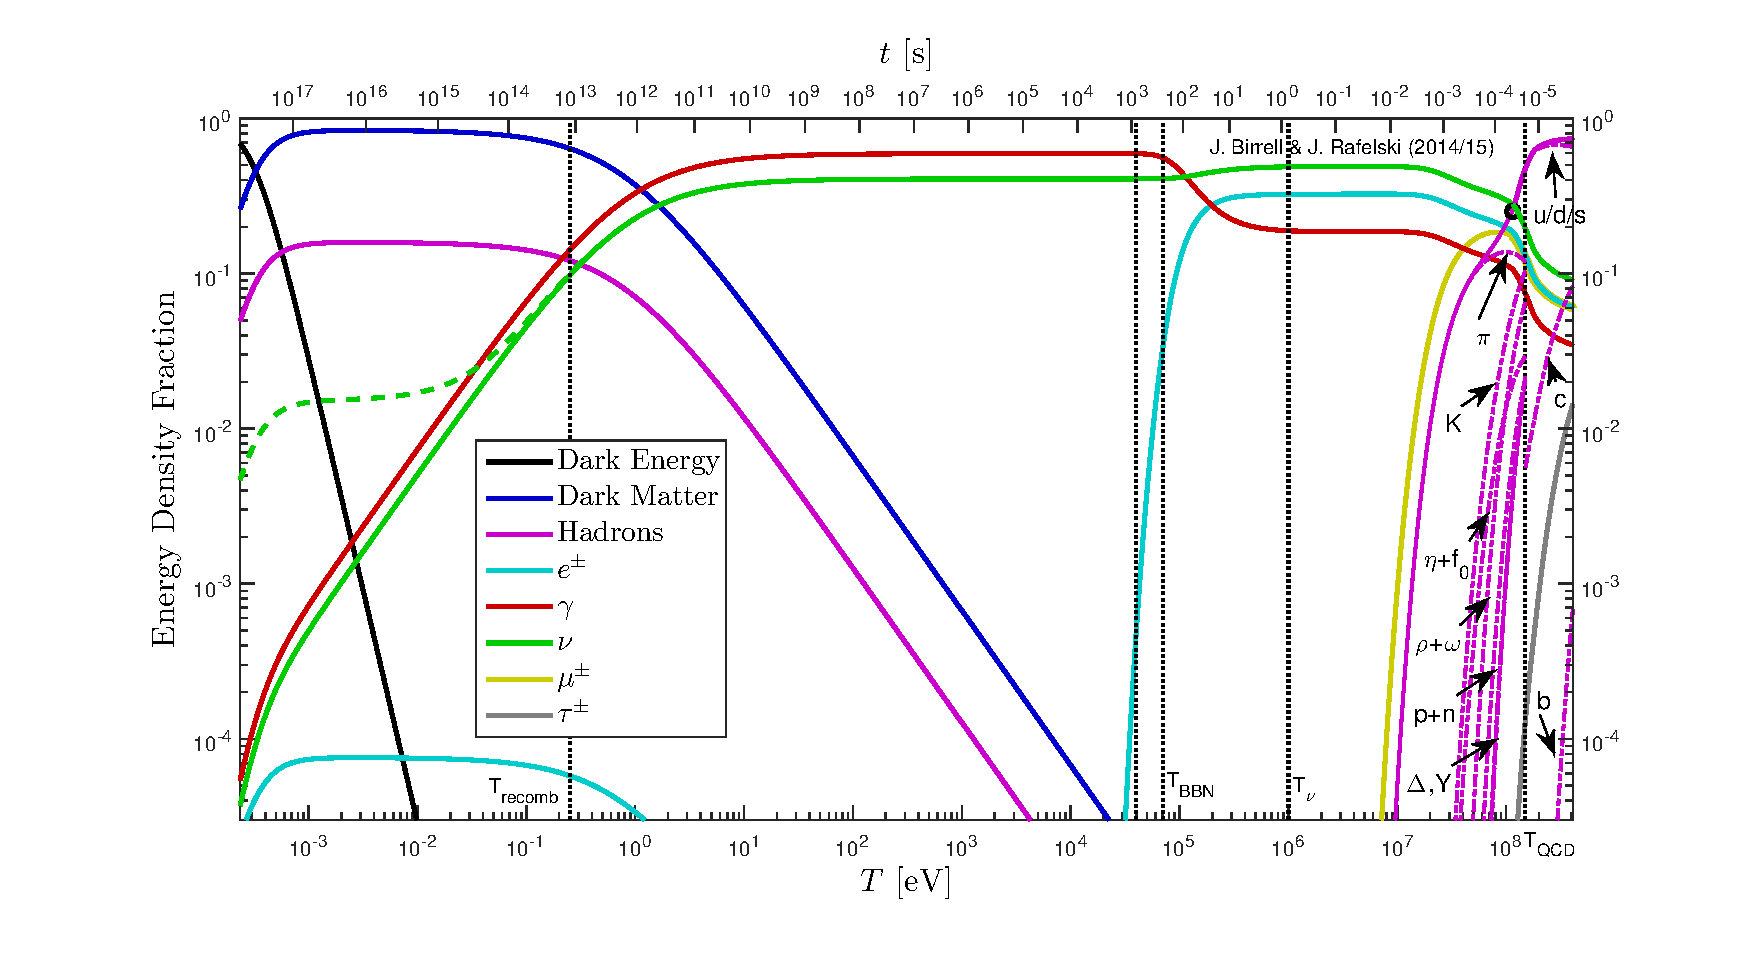
\includegraphics[height=11cm]{./plots/energy_fractions.eps}}
  \centerline{\hspace*{0.4cm}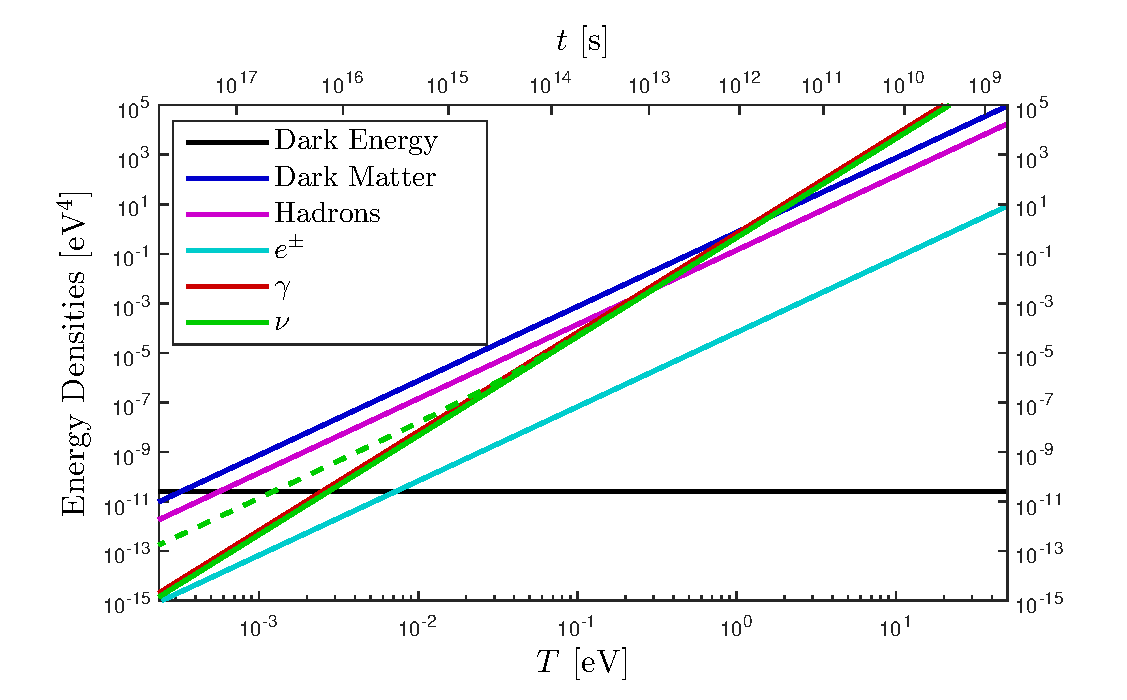
\includegraphics[height=8.5cm]{./plots/energy_densities.eps}}
  \caption{Current era: $69\%$ dark energy, $26\%$ dark matter, $5\%$ baryons, $<1\%$ photons and neutrinos.  Solid neutrino line shows massless neutrinos while the dashed line shows $1$ massless and $2\times 0.1$ eV neutrinos (Neutrino mass choice is just for illustration.  Other values are possible).\label{fig:energy_frac}}
   \end{figure}
%%%%%%%%%%%%%%%%%%%%%%%%%%%%%%%%%%%%%%%

The universe is filled with magnetic fields at various scales and strengths both within galaxies and in deep extra-galactic space far and away from matter sources. Extra-galactic magnetic fields are not well constrained today, but are required by observation to be non-zero with a magnitude between $10^{-12}\ \mathrm{T}>B_{EGMF}>10^{-20}\ \mathrm{T}$ over Mpc coherent length scales. The upper bound is constrained from the characteristics of the CMB while the lower bound is constrained by non-observation of ultra-energetic photons from blazars. There are generally considered two possible origins for extra-galactic magnetic fields: (a) matter-induced dynamo processes involving Amperian currents and (b) primordial (or relic) seed magnetic fields whose origins may go as far back as the Big Bang itself. It is currently unknown which origin accounts for extra-galactic magnetic fields today or if it some combination of the two models. Even if magnetic fields in the universe today are primarily driven via amplification through Amperian matter currents, such models still require primordial seed fields at some point to act as catalyst.

At an early time in the standard cosmology model, the universe began as a fireball with extremely high temperature and high energy density. The ultrarelativistic plasma produced in the early universe then underwent several phases changes which changed gross properties as the universe expanded and cooled. The comic plasma, after the electroweak symmetry breaking epoch and presumabely inflation, occured in the early universe in the following sequence:
\begin{itemize}
  \item Primordial quark-gluon plasma: At early times when the temperature was between $130\ \mathrm{GeV}>T>150\ \mathrm{MeV}$, we have leptons, gauge mesons, and deconfined quarks which propagated freely and all hadrons are dissolved into their constituents. At that time, strongly interacting nearly massless particles $u,d,s,G$ controlled the fate of the universe.
  \item Hadronic plasma: Around the hadronization temperature $T_h\approx150\ \mathrm{MeV}$, a phase transformation occured forcing the stongly interacting particles such as quarks and gluons to condense into confined states. It is here where matter as we know it today forms and the universe becomes hadronic-matter dominated. In the temperature range $ 60\ \mathrm{MeV}>T>20\ \mathrm{MeV}$ the universe is rich in physics phenomena involving strange mesons and (anti)baryons including (anti)hyperon abundances \cite{Fromerth:2012fe,Yang:2021bko}.
  \item  Electroweak plasma: For temperature $10\ \mathrm{MeV}>T>1\ \mathrm{MeV}$, the universe contained relativistic electrons, positrons, photons, and three species of neutrinos/antineutrinos. In this range, neutrinos were still coupled to the charged leptons via the weak interaction, and the properties of the universe are controlled by this electroweak plasma \cite{Birrell:2012gg}.
  \item  Electron-positron plasma: After neutrinos decoupled and become free-streaming, referred to as neutrino freezeout, from the cosmic plasma at $T=1\ \mathrm{MeV}$, the cosmic plasma was dominated by electrons, positrons, and photons. We have shown in \cite{Chris:2023abc} that this plasma existed until $T\approx0.02\ \mathrm{MeV}$ such that BBN occured within a rich electron-positron plasma.
  \item Electron-proton plasma: The final major plasma stage in the universe began after the annihilation of the majority of $e^{\pm}$ pairs leaving behind a residual amount of electrons determined by the baryon asymmetry in the universe and charge conservation. The universe was still opaque to photons at this point and remained so until the recombination period at $T\approx0.26\ \mathrm{eV}$ starting the era of observational consmology with the CMB.
\end{itemize}
%%%%%%%%%%%%%%%%%%%%%%%%%%%%%%%%%%%%%%%
\begin{figure}[h]
  %\begin{center}
  \centering
  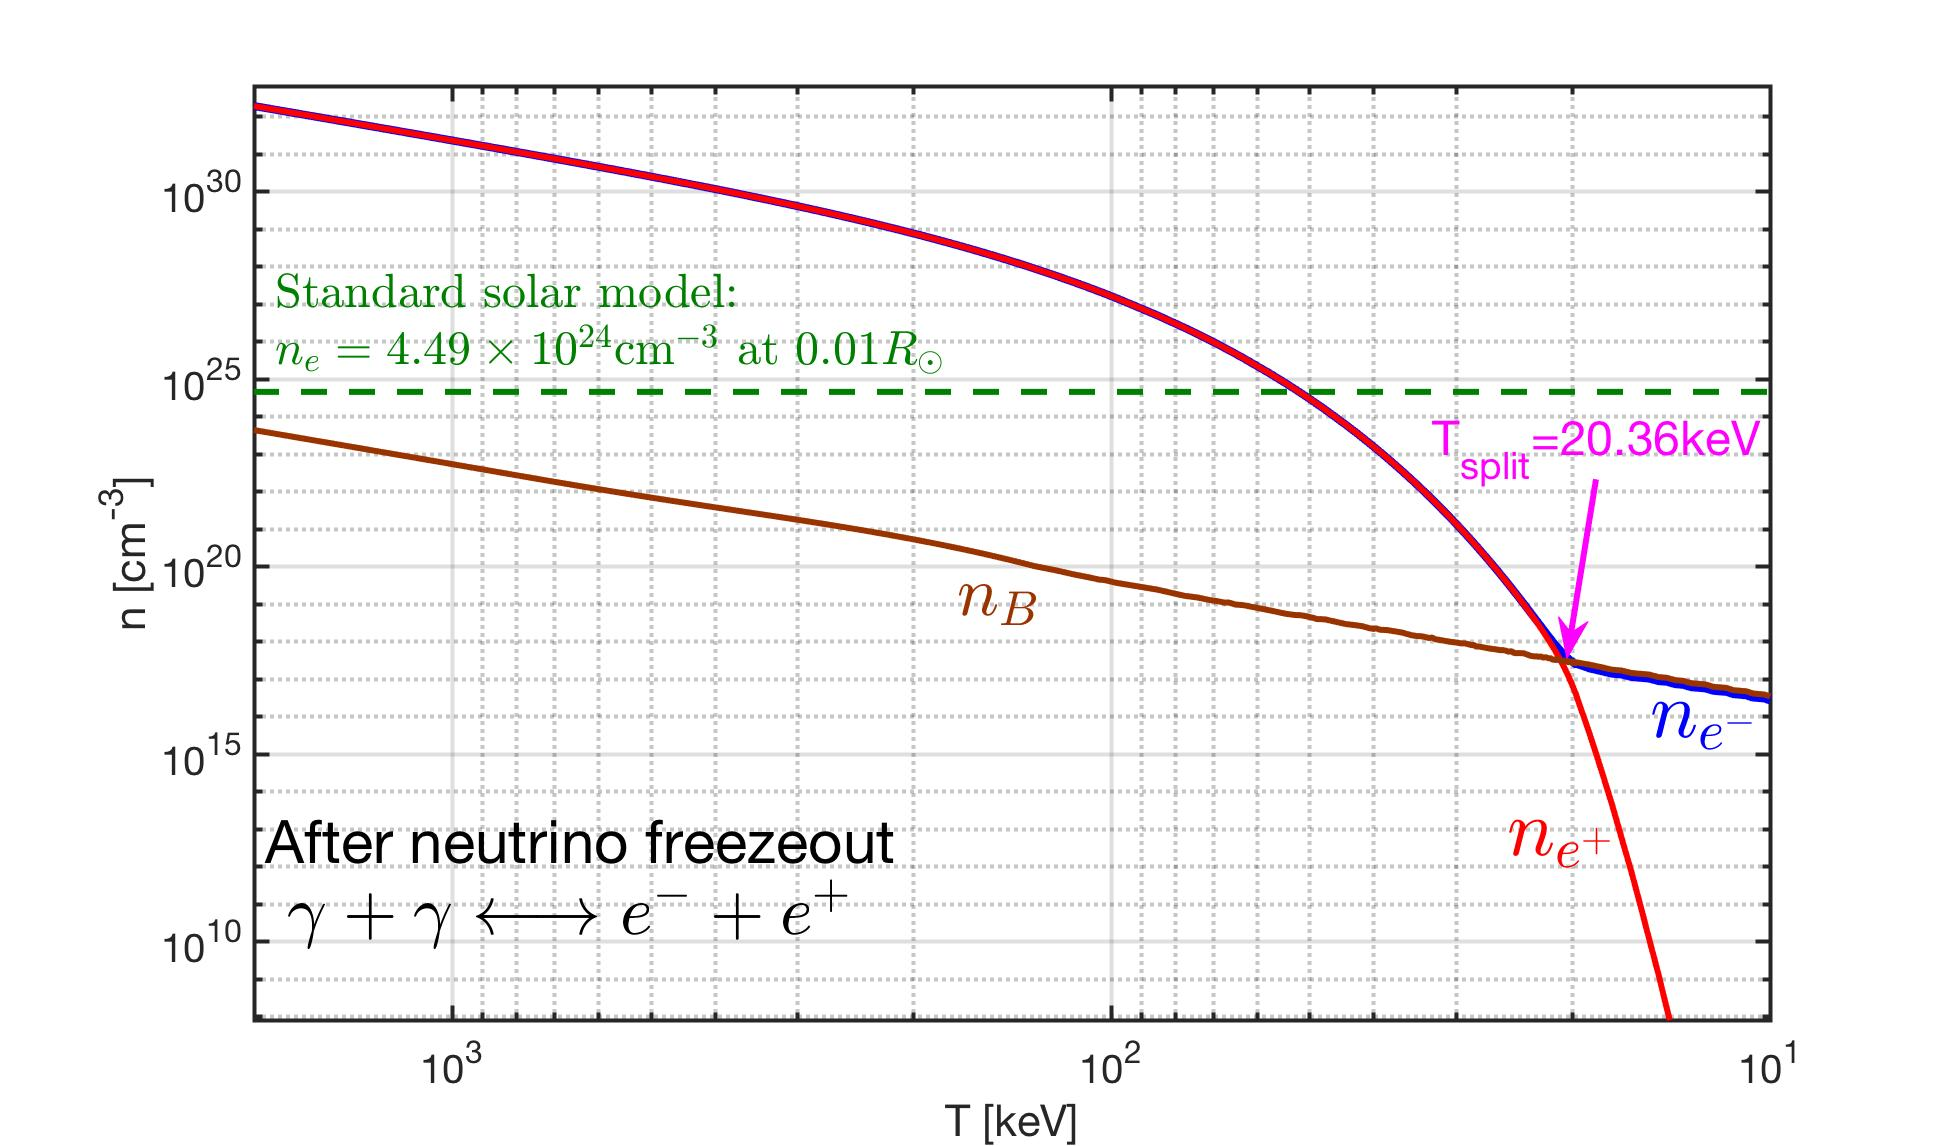
\includegraphics[width=0.75\linewidth]{./plots/NewDensity_cm3.jpg}
  \caption{The electron(positron) number density as a function of temperature in the range $2\,\mathrm{MeV}>T>10\,\mathrm{keV}$. The blue solid line is the electron density, the red solid line is the positron density, and the brown solid line is the baryon density. For comparison, we also show the green dotted line as the solar electron density within the stellar core. This reveals we have an electron-positron rich plasma in early universe until $T_{\mathrm{split}} = 20.36\ \mathrm{keV}$, for $T<T_{\mathrm{split}}$ the positron density quickly vanishes because of annihilation leaving only a residual electron density as required by charge conservation.}
  \label{Density_fig} 
\end{figure}
%%%%%%%%%%%%%%%%%%%%%%%%%%%%%%%%%%%%%%%
The properties of the electron-positron $e^{\pm}$ plasma in the early universe has not received appropriate attention in an era of precision BBN studies~\cite{Pitrou:2018cgg}. The presence of $e^{\pm}$ pairs before and during BBN has been acknowledged by Wang, Bertulani and Balantekin~\cite{Wang:2010px} over a decade ago. This however was before necessary tools were developed to explore the connection between electron and neutrino plasmas~\cite{Mangano:2005cc,Birrell:2012gg,Birrell:2014uka}. 

In \rf{Density_fig} we show that the dense $e^{\pm}$ plasma in early universe under the hypothesis charge neutrality and entropy conservation as a function of temperature $2\,\mathrm{MeV}>T>10\,\mathrm{keV}$ \cite{Chris:2023abc}. The plasma is electron-positron rich, i.e, $n_{\pm}\gg n_B$ in the early universe until leptonic annihilation at $T_{\mathrm{split}} = 20.36\ \mathrm{keV}$. For $T<T_{\mathrm{split}}$ the positron density $n_{e^+}$ decreases dramatically because of annihilation and the residual electron density becomes equal to the proton density in accordance with charge neutrality in the universe as a whole.
\begin{figure}[htbp]
  \centering
  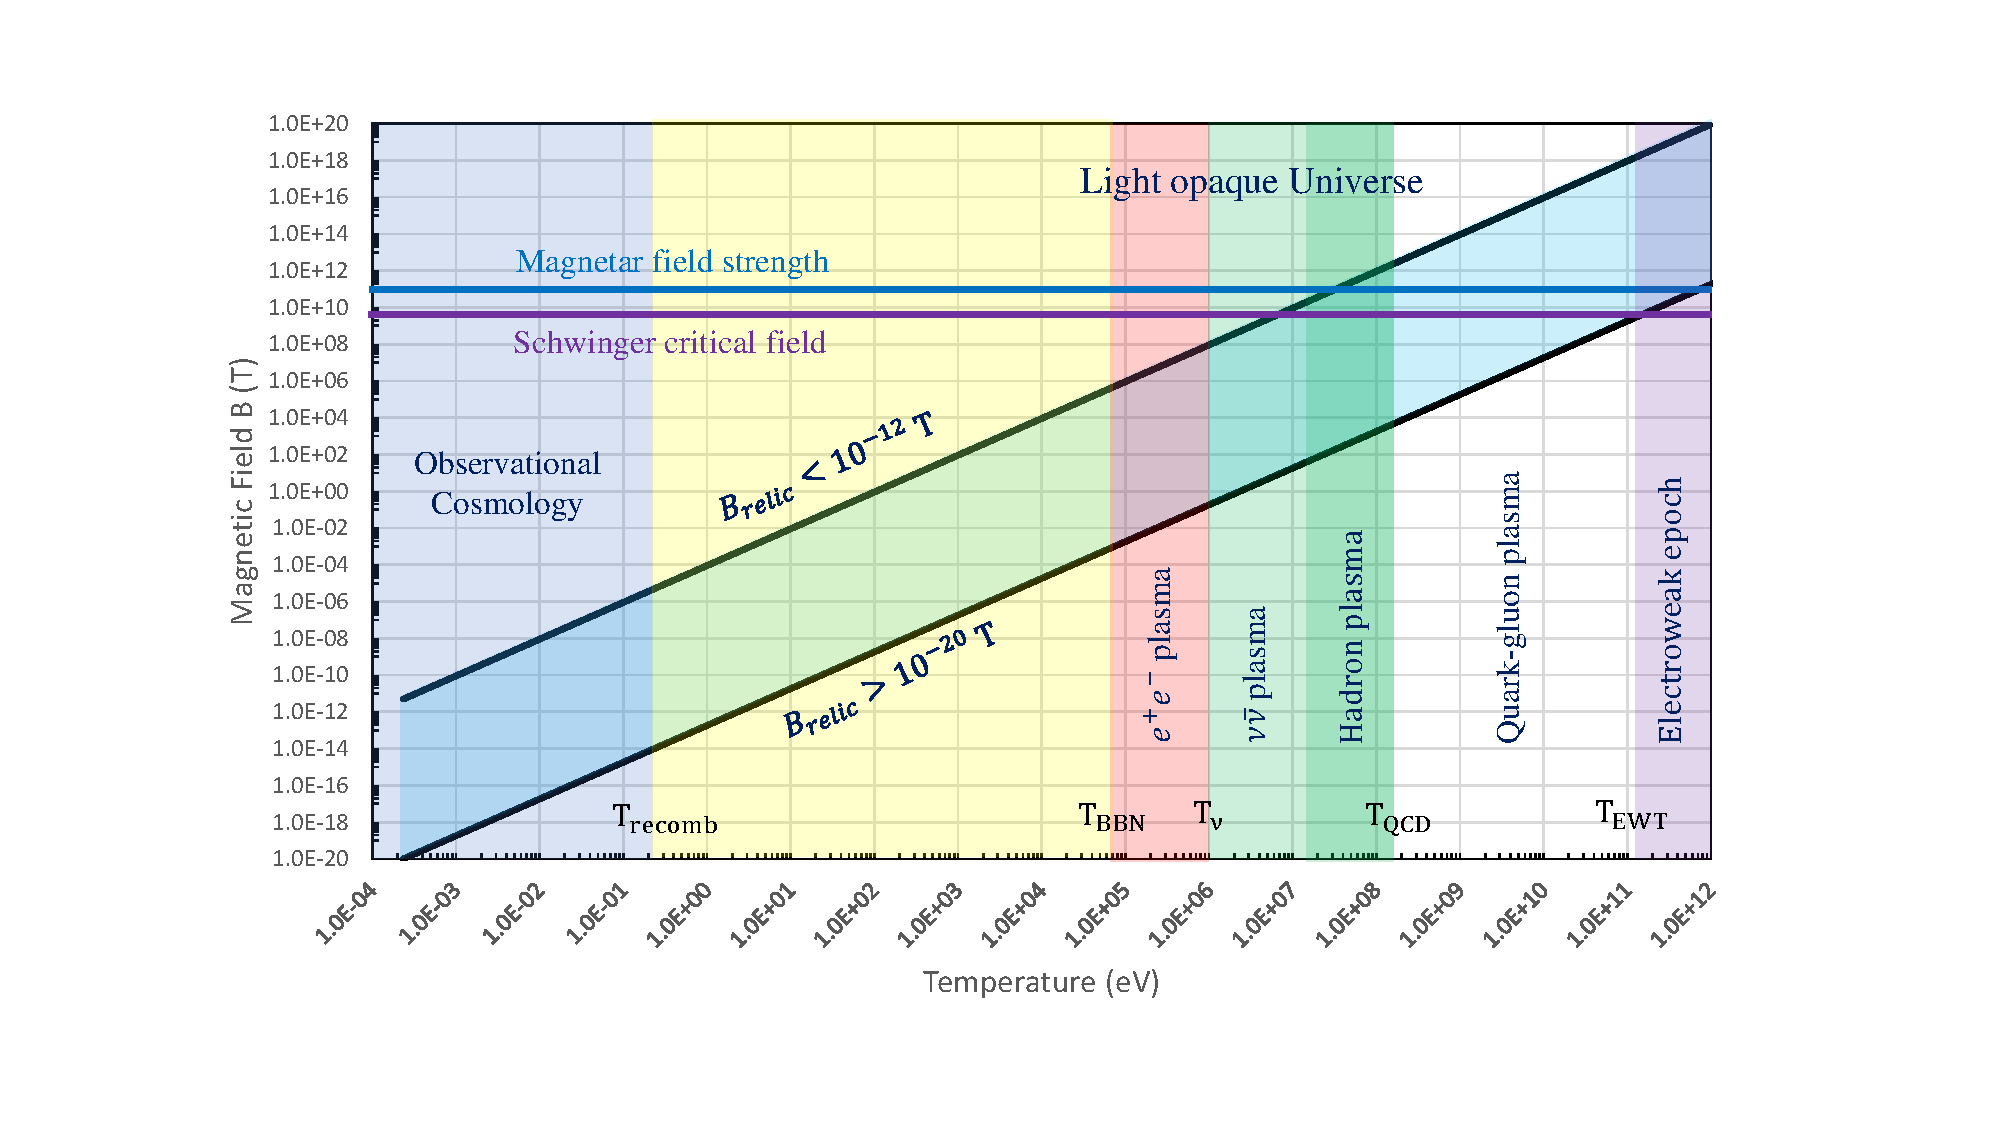
\includegraphics[trim=110 50 120 40,clip,width=\textwidth]{./plots/relic_plot.PDF}
  \label{relic_plot}
  \caption{Qualitative value of the primordial magnetic field over the evolutionary lifespan of the universe. As magnetic flux is conserved over co-moving surfaces, the primordial relic field is expected to dilute as $B\propto1/a(t)^{2}$ meaning the contemporary small bounded values of $5\times10^{-12}\ \mathrm{T}>B_{relic}>10^{-20}\ \mathrm{T}$ may have once represented large magnetic fields in the early universe. This is relic magnetic field would then be generated by the last phase of significant magnetization in the early universe. This figure is meant to be illustrative and it is unlikely the magnetization of the universe would proceed unhindered and unaltered into the ultra-dense plasma phases of the early universe. The values of the Schwinger critical field and the upper bound of surface magnetar field strength are included for scale.}
\end{figure}

We can now connect back to the consideration of cosmic magnetic fields as they might have risen in the environment of early universe plasmas noting that such primordial magnetic fields would be lensed through each of the various plasmas that existed when the universe was far hotter and denser. Of particular interest to us is the electron-positron plasma which existed in the early universe especially at temperatures $T>35\ \mathrm{keV}$ which was the last matter(antimatter) plasma in the universe where the energy its density exceeded that of the proton/neutron baryon energy density. This dense plasma environment is where BBN occurred and where similar plasmas can still be found within exotic stars such as magnetars. The contemporary relic magnetic fields may then be an artifact of this final time of universe-scale magnetization in a manner similar to how the CMB is a relic of the time of charge recombination.

%%%%%%%%%%%%%%%%%%%%%%%%%%%%%%%%%%%%%%%%%%%%%%%%%%%%%%%%%%%%%%%%%%%
\section{Energy Eigenvalues}\label{sec:energy}
\noindent As a starting point, we consider the energy eigenvalues of charged fermions within a homogeneous magnetic field. Here, we have several choices: We could assume the typical Dirac energy eigenvalues with gyro-magnetic g-factor set to $g=2$. But as electrons, positrons and most plasma species have anomalous magnetic moments (AMM), we require a more complete model. Another option would be to modify the Dirac equation with a Pauli term, often called the Dirac-Pauli (DP) approach, via
\begin{align}
  \label{Pauli} \hat{H}_{\mathrm{AMM}} = -a\frac{e}{2m_{e}}\frac{\sigma_{\mu\nu}F^{\mu\nu}}{2}\,,
\end{align}
where $\sigma_{\mu\nu}$ is the spin tensor proportional to the commutator of the gamma matrices and $F^{\mu\nu}$ is the EM field tensor. For the duration of this work, we will remain in natural units $(\hbar=c=k_{B}=1)$ unless explicitly stated otherwise. The AMM is defined via g-factor as
\begin{align}
  \label{AMM} \frac{g}{2}=1+a\,.
\end{align}
This approach, while straightforward, would complicate the energies making analytic understanding and clarity difficult without a clear benefit. Our preferred model for the AMM is through the Klein-Gordon-Pauli (KGP) equation which is given by
\begin{alignat}{1}
  \label{KGP} \left(\left(i\partial_{\mu}-eA_{\mu}\right)^{2}-m_{e}^{2}-e\frac{g}{2}\frac{\sigma_{\mu\nu}F^{\mu\mu}}{2}\right)\Psi=0\,.
\end{alignat}
We wish to emphasize, that each of the three above models are distinct and have differing physical consequences and are not interchangeable. One benefit of the KGP approach is that the energies take eigenvalues which are mathematically similar to the Dirac energies. Considering the $e^\pm$ plasma in a uniform magnetic field $B$ pointing along the $z$-axis, the energy of $e^\pm$ fermions can be written as
\begin{align}
  \label{KGPEnergy} E_{n}^{s}&=\sqrt{p^2_z+\tilde{m}^2+2eBn},\qquad\tilde{m}^2=m^2_e+eB\left(1-gs\right),\qquad s=\pm\frac{1}{2},\qquad n=0,1,2,3,\dots
\end{align}
where $n$ is the principle quantum number for the Landau levels and $s$ is the spin quantum number. Here we introduce a notion of \lq\lq magnetic mass\rq\rq\ which inherits the spin-specific part of the energy adding them to the mass. This convention is also generalizable to further non-minimal electromagnetic models with more exotic energy contributions such that we write a general replacement as
\begin{align}
  \label{MagMass} m_{e}^{2}\rightarrow\tilde{m}^2(B)\,.
\end{align}
This definition also pulls out the ground state Landau energy separating it from the remainder of the Landau tower of states. One restriction is that the magnetic-mass must remain positive definite in our analysis thus we require
\begin{align}
  \label{MassLimit} \tilde{m}^2(B)=m^2_e+eB\left(1-gs\right)>0\,.
\end{align}
This condition fails under ultra-strong magnetic fields of order
\begin{align}
  \label{MagMassFail} B_{\mathrm{crit}}=\frac{m_{e}^{2}}{ea}=\frac{\mathcal{B}_{S}}{a}\approx3.8\times10^{12}\ \mathrm{T}\,,
\end{align}
where $\mathcal{B}_{S}$ is the Schwinger critical field strength. For electrons, this field strength is well above the window of magnetic field strengths of interest during the late $e^{\pm}$ epoch.

%%%%%%%%%%%%%%%%%%%%%%%%%%%%%%%%%%%%%%%%%%%%%%%%%%%%%%%%%%%%%%%%%%
\section{Landau eigen-energies in cosmology}
\noindent The standard model of cosmology with a cosmological constant plus cold dark matter ($\Lambda\mathrm{CDM}$) is described by the Friedman-Lemaître-Robertson-Walker (FLRW) metric. The spatially flat (Gaussian curvature $k=0$) FLRW metric with metric signature $(+1,-1,-1,-1)$ in Cartesian coordinates is
\begin{align}
    \label{FLRW} ds^2=dt^2-a^2(t)\left[dx^2+dy^2+dz^2\right]\,.
\end{align}
The scale factor $a(t)$ denotes the change of proper distances in an expanding (or contracting) universe which is both homogeneous and isotropic. The evolutionary expansion of the universe is then traditionally defined in terms of the Hubble parameter $H$ as follows
\begin{align}
    \label{FriedmannOne}H^2\equiv\left(\frac{\dot a}{a}\right)^2=\frac{8\pi G_N}{3}\rho_{tot}
\end{align}
where $G_N$ is the Newtonian constant of gravitation and $\rho_{tot}$ is the total energy density of the universe. \req{FriedmannOne} is also known as the first Friedmann equation. 

There is another natural scale for the magnetic field besides \req{MagMassFail} when considering the consequences of FLRW expansion on the $e^{\pm}$ fluid. As the universe expands, different terms in the energies and thus partition function evolve as a function of the scale factor $a(t)$ which arises in the FLRW metric. We can consider the expansion to be an adiabatic process which results in a smooth shifting of the relevant dynamical quantities. From the conservation of magnetic flux through a co-moving surface, the magnetic field under expansion starting at some initial time $t_{0}$ is given by
\begin{alignat}{1}
    \label{BScale} B(t) = B(t_{0})\frac{a(t_{0})^{2}}{a(t)^{2}}\,.
\end{alignat}
As the universe expands, the temperature also cools as the cosmological redshift reduces the kinetic energies of particles in the universe lowering their contribution to the energy content of the universe. This cosmological redshift is written as
\begin{alignat}{1}
    \label{TScale} T(t) = T(t_{0})\frac{a(t_{0})}{a(t)}\,.
\end{alignat}
The momenta scale with the same factor as temperature, which is the origin of cosmological redshift
\begin{alignat}{1}
    \label{PScale} p_{i}(t) = p_{i}(t_{0})\frac{a(t_{0})}{a(t)}\,.
\end{alignat}
The energy of massive free particles in the universe scales differently based on their momentum (and thus temperature). When hot and relativistic, particle energy scales with inverse scale factors like radiation. However as particles transition to non-relativistic momenta, their energies scale with the inverse square of the scale factor like magnetic flux.
\begin{alignat}{1}
    \label{EScale} E(t) = E(t_{0})\frac{a(t_{0})}{a(t)}\xrightarrow{\mathrm{NR}}\  E(t_{0})\frac{a(t_{0})^{2}}{a(t)^{2}}\,.
\end{alignat}
This occurs because of the functional dependence of energy on momentum in the relativistic versus non-relativistic cases. The argument in the Boltzmann statistical factor is given by
\begin{alignat}{1}
    \label{Boltz} X_{n}^{s}\equiv\frac{E_{n}^{s}}{T}\,.
\end{alignat}
We can explore this relationship for the magnetized system explicitly by writing out \req{Boltz} using the KGP eigen-energies as
\begin{alignat}{1}
    \label{XExplicit} X_{n}^{s} = \sqrt{\frac{m_{e}^{2}}{T^{2}}+\frac{p_{z}^{2}}{T^{2}}+\frac{2eB}{T^{2}}\left(n+\frac{1}{2}-\frac{gs}{2}\right)}\,,
\end{alignat}
where we now introduce the expansion scale factor via \req{BScale} - \req{PScale}. The Boltzmann factor can then be written as
\begin{alignat}{1}
    \label{XScale} X_{n}^{s}[a(t)] = \sqrt{\frac{m_{e}^{2}}{T^{2}(t_{0})}\frac{a(t)^{2}}{a(t_{0})^{2}}+\frac{p_{z}^{2}(t_{0})}{T^{2}(t_{0})}+\frac{2eB(t_{0})}{T^{2}(t_{0})}\left(n+\frac{1}{2}-\frac{gs}{2}\right)}\,.
\end{alignat}
This reveals that only the mass contribution is dynamic over cosmological time. For any given eigen-state, the mass term increases driving the state into the non-relativistic limit while the momenta and magnetic contributions are frozen by initial conditions. As a point of comparison, the Boltzmann factor for the DP eigen-energies becomes
\begin{alignat}{1}
    \label{XDP} X_{n}^{s}\vert_{DP} = \sqrt{\left(\sqrt{\frac{m_{e}^{2}}{T^{2}}+\frac{2eB}{T^{2}}\left(n+\frac{1}{2}-s\right)}-\frac{eB}{2mT}(g-2)s\right)^{2}+\frac{p_{z}^{2}}{T^{2}}}\,,
\end{alignat}
which over cosmological time under expansion scales as
\begin{alignat}{1}
    \label{XScaleDP} X_{n}^{s}[a(t)]\vert_{DP} = \sqrt{\left(\sqrt{\frac{m_{e}^{2}}{T^{2}(t_{0})}\frac{a(t)^{2}}{a(t_{0})^{2}}+\frac{2eB(t_{0})}{T^{2}(t_{0})}\left(n+\frac{1}{2}-s\right)}-\frac{eB(t_{0})}{2mT(t_{0})}\frac{a(t_{0})}{a(t)}(g-2)s\right)^{2}+\frac{p_{z}^{2}(t_{0})}{T^{2}(t_{0})}}\,.
\end{alignat}
We note here one important difference between KGP and DP eigen-energies in the context of cosmology: The anomalous magnetic moment portion of the DP statistics is suppressed by $1/a(t)$ over cosmological time while the AMM contribution is preserved in the KGP model. That the universe's expansion makes a distinction between $g=2$ magnetic moment and AMM for DP fermions appears as a rather artificial and nonphysical trait. While the suppression of AMM may often be small for particles such as electrons, this suppression is non-trivial for particles with large AMM values such as the proton. That cosmological redshift would push DP protons to be described by $g=2$ eign-energies in the non-relativistic limit counts as a malaise for the model and further strengthens our thinking that the KGP model is more appropriate for cosmological studies. Motivated by \req{XScale}, we can introduce a dimensionless cosmic magnetic scale which is frozen in the homogeneous case as
\begin{alignat}{1}
    \label{Bo} b_{0}\equiv\frac{eB}{T^{2}}=\frac{eB\hbar c^{2}}{(k_{B}T)^{2}}\ \mathrm{(S.I)}\,,
\end{alignat}
where we've included the expression explicitly in full SI units. We can estimate the value of $b_{0}$ from the bounds on the extra-galactic magnetic field strength and the temperature of the universe today.  If the origin of deep space extra-galactic magnetic fields are relic fields from the early universe, which today are expected to exist between $5\times10^{-12}\ \mathrm{T}>B_{relic}>10^{-20}\ \mathrm{T}$, then at temperature $T=2.7\ \mathrm{K}$, the value of the cosmic magnetic scale is between
\begin{alignat}{1}
    \label{BoScale} 5.5\times10^{-5}>b_{0}>1.1\times10^{-11}\,.
\end{alignat}
This should remain constant in the universe at-large up to the last epoch the universe was sufficiently magnetized to disturb this value. As the electron-proton plasma which generated the CMB was relatively dilute over its duration, it was unlikely sufficiently magnetized to significantly alter this value over extra-galactic scales. Rather, the best candidate plasma to have been sufficiently magnetized and dense to have set the relic field magnetic scale would have been the electron-positron plasma which existed during the duration of Big Bang Nucleosynthesis (BBN) and beforehand.

Higher order non-minimal magnetic contributions which can be introduced via \req{MagMass} to the eigen-energies like $\approx\mu_{B}^{2}B^{2}/T^{2}$ are even more surpressed over cosmological time which drives the system into minimal electromagnetic coupling with the exception of the anomalous magnetic moment in the KGP case. It is interesting to note that cosmological expansion serves to \lq\lq smooth out\rq\rq\ the characteristics of more complex BSM electrodynmaics erasing them from a statistical perspective in favor of the minimal or minimal-like dynamics. As $b_0$ is a constant of expansion, assuming the electron-proton plasma between the CMB and electron-positron annihilation did not greatly disturbed it, we can calculate the remnant values at the temperature $T=50\ \mathrm{keV}$ with the expression
\begin{align}
  \label{BBNFields} B(T)=\frac{b_{0}}{e}T^{2}\,,
\end{align}
yielding a range of field strengths
\begin{align}
  \label{BBNRange} 2.3\times10^{5}\ \mathrm{T}>B(T=50\ \mathrm{keV})>4.6\times10^{-4}\ \mathrm{T}\,,
\end{align}
during which the electron-positron plasma in the universe had a number density comparable to that of the Solar core with $n_{e}=4.49\times10^{24}\ \mathrm{cm}^{-3}$ at $r=0.01R_{\odot}$.

%%%%%%%%%%%%%%%%%%%%%%%%%%%%%%%%%%%%%%%%%%%%%%%%%%%%%%%%%%%%%%%%%%%
\section{Partition function}
\noindent We now turn our attention now to the statistical behavior of the $e^{\pm}$ system. We can utilize the general fermion partition function given by
\begin{align}
  \label{PartFunc} \ln\mathcal{Z}=\sum_{\alpha}\ln\left(1+e^{-\beta(E-\eta)}\right)\,,
\end{align}
where $\beta=1/T$, $\alpha$ is the set of all quantum numbers in the system, and $\eta$ is the generalized chemical potential. The magnetized $e^{\pm}$ system should be considered a system of four quantum species: Particles and anti-particles, and spin aligned and anti-aligned. Taken together we consider a system where all electrons and positrons are spin aligned or anti-aligned with the magnetic field $B$ and the partition function of the system is written as
\begin{align}
\ln\mathcal{Z}_{tot}=\frac{2eBV}{(2\pi)^2}\sum_{n=0}^\infty\int^\infty_{0} \!\!dp_z\bigg[&\ln\left(1+ e^{-\beta(E_{n}^+-\eta_{e}-\eta_s)}\right)+\ln\left(1+e^{-\beta(E_{n}^--\eta_{e}+\eta_s)}\right)\notag\\
&+\ln\left(1+e^{-\beta(E_{n}^++\eta_{e}+\eta_s)}\right)+\ln\left(1+e^{-\beta(E_{n}^-+\eta_{e}-\eta_s)}\right)\bigg],
\end{align}
where $\eta_{e}$ is the electron chemical potential and $\eta_s$ is the spin chemical potential%and the positron chemical potential is the negative of the electron's 
and energy $E_{n}^\pm$ can be written as
\begin{align}
E_{n}^\pm&=\sqrt{p^2_z+\tilde m^2_\pm+2eBn},\qquad\tilde{m}^2_\pm=m^2_e+eB\left(1\mp\frac{g}{2}\right)\,,
\end{align}
where the $\pm$ script refers to spin aligned and anti-aligned eigenvalues. To simplify the partition function we consider the case $\eta_s/T\ll1$ for the first approximation and use the expansion of the logarithmic function into a power series yielding
\begin{align}
\ln\left(1+x\right)=\sum^{\infty}_{k=1}\frac{(-1)^{k+1}}{k}x^k, \,\,\,\,\,\,\,\mathrm{for}\,|x|<1.
\end{align}
We emphasize that this expansion is only value where the Boltzmann factor $\exp\left(-\beta(E\pm\eta_{e})\right)$ remains less than unity, otherwise the partition function becomes divergent and ill-behaved. The partition function of $e^{\pm}$ system can be further expanded to isolate the contribution of the chemical potential $\eta_{e}$ as
\begin{align}
  \label{PartTotal}\ln\mathcal{Z}_{tot}
  &=\frac{2eBV}{(2\pi)^2}\sum_{n=0}^\infty\sum^{\infty}_{k=1}\frac{(-1)^{k+1}}{k}\bigg[e^{k\beta\eta_{e}}+e^{-k\beta\eta_{e}}\bigg]\left(\int_0^\infty dp_z\,e^{-k\beta E_n^+}+\int_0^\infty dp_z\,e^{-k\beta E_n^-}\right)\notag\\
  &=\frac{2eBTV}{(2\pi)^2}\sum^{\infty}_{k=1}\frac{(-1)^{k+1}}{k^2}\bigg[2\cosh{(k\beta\eta_{e})}\bigg]\sum_{n=0}^\infty \left(W^+_1(n,k)+ W^-_1(n,k)\right),
\end{align}
where we introduce the function $W^\pm_1(n,k)$ as follows
\begin{align}
W^\pm_1(n,k)\equiv\frac{k\sqrt{\tilde{m}^2_\pm+2eBn}}{T}\,\,K_1\!\!\left(\frac{k\sqrt{\tilde{m}^2_\pm+2eBn}}{T}\right),
\end{align}
defined in terms of the modified (hyperbolic) Bessel function of the second kind $K_{i}(x)$. We then utilize the Euler-Maclaurin formula to replace the sum over Landau levels with an integration yielding
\begin{align}
  \label{EMIntegration}\sum^{\infty}_{n=0}W^\pm_1(n,k)=\int^\infty_0\!\!dn\,W^\pm_1(n,k)+\frac{1}{2}\bigg[W^\pm_1(\infty,k)+W^\pm_1(0,k)\bigg]+\frac{1}{12}\bigg[\left.\frac{\partial W^\pm_1}{\partial n}\right|_{\infty}-\left.\frac{\partial W^\pm_1}{\partial n}\right|_{0}\bigg]+R\,,
\end{align}
where $R$ is the error remainder which is defined by integrals over Bernoulli polynomials. The error remainder has, for well behaved functioned, a finite size and therefore for a more extensive analysis is required to demonstrate to what order in Bessel functions is required to minimize the error remainder for good results. For \req{EMIntegration}, we've chosen to include up to the first order in derivatives. Using the asymptotic properties of Bessel function $K_{i}(x)$ as $x$ becomes large, we can simplify the above expression to obtain
\begin{align}
  \label{Winitial}\sum^{\infty}_{n=0}W^\pm_1(n,k)&=\int^\infty_0\!\!dn\,W^\pm_1(n,k)+\frac{1}{2}W^\pm_1(0,k)-\frac{1}{12}\left.\frac{\partial W^\pm_1}{\partial n}\right|_{0}+R\\
  \label{WReplacement}
  &=\left(\frac{T^2}{k^2eB}\right)x_{\pm}^{2}K_{2}(x_{\pm})+\frac{1}{2}x_{\pm}K_{1}(x_{\pm})+\frac{1}{12}\left(k^2b_0\right)K_{0}(x_{\pm})+R\,,\qquad x_{\pm} = \frac{k\tilde{m}_{\pm}}{T}\,.
\end{align}
Here we see mathematically that the ground state $n=0$, which has no analogue in the classical continuum limit, contributes to a difference between the sum and integral formulations. Replacing the sum over Landau levels by the integral, the partition function can separated into three distinct parts
\begin{align}
  \ln\mathcal{Z}_{tot}=\ln\mathcal{Z}_{free}+\ln\mathcal{Z}_B+\ln\mathcal{Z}_R\,,
\end{align}
where we define 
\begin{align}
  \label{FreePart}&\ln\mathcal{Z}_{free}=\frac{T^3V}{2\pi^2}\sum^{\infty}_{k=1}\frac{(-1)^{k+1}}{k^4}\left[2\cosh{\left(\frac{k\eta_{e}}{T}\right)}\right]\sum_{i=\pm}x_i^2K_2\left(x_i\right)\,,\\
  \label{MagPart}&\ln\mathcal{Z}_B=\frac{eBTV}{2\pi^2}\sum^{\infty}_{k=1}\frac{(-1)^{k+1}}{k^2}\left[2\cosh{\left(\frac{k\eta_{e}}{T}\right)}\right]\sum_{i=\pm}\bigg[\frac{x_i}{2}K_1\left(x_i\right)+\frac{k^2b_0}{12}K_0\left(x_i\right)\bigg]\,,\\
  \label{ErrorPart}&\ln\mathcal{Z}_R=\frac{eBTV}{\pi^2}\sum^{\infty}_{k=1}\frac{(-1)^{k+1}}{k^2}\left[2\cosh{\left(\frac{k\eta_{e}}{T}\right)}\right]R.
\end{align}
While this would require further derivation to demonstrate explicitly, the benefit of the Euler-Maclaurin approach is if the error contribution remains finite or bound for the magnetized partition function, then a correspondence between the free Fermi partition function (with noticeably modified magnetic-mass $\tilde{m}_{\pm}$) and the magnetized Fermi partition function can be established. The mismatch between the summation and integral in the Euler-Maclaurin formula would then encapsulate the immediate magnetic response and deviation from the free particle phase space.

%%%%%%%%%%%%%%%%%%%%%%%%%%%%%%%%%%%%%%%%%%%%%%%%%%%%%%%%%%%%%%%%%%%
\subsection{Non-relativistic limit of the partition function}
While we label $\ln(\mathcal{Z}_{free})$ in \req{FreePart} as the \lq\lq free\rq\rq\ partition function, this is not strictly true as this contribution to the overall partition function is a function of the magnetic-mass we defined earlier in \req{MagMass}. When determining the magnetization of the quantum Fermi gas, derivatives of the magnetic field $B$ will not fully vanish on this first term which will resulting in an intrinsic magnetization which is distinct from the contribution from the ground state and mismatch between the quantized Landau levels and the continuum of the free momentum. Specifically, this free Fermi contribution represents the magnetization that arises from the spin magnetic energy rather than orbital contributions. To demonstrate this, we will briefly consider the weak field limit for $g=2$. The magnetic-mass, for $g=2$, have the following values
\begin{align}
  \label{MagMassPlus} \tilde{m}_{+}^{2}&=m_{e}^{2}\,,\\
  \label{MagMassMinus} \tilde{m}_{-}^{2}&=m_{e}^{2}+2eB\,.
\end{align}
The energy eigenvalues are then
\begin{align}
  \label{EPlus} E_{n}^{+}=\sqrt{p_{z}^{2}+m_{e}^{2}+2eBn}\,,\\
  \label{EMinus} E_{n}^{-}=\sqrt{\left(E_{n}^{+}\right)^{2}+2eB}\,,
\end{align}
The spin anti-aligned energies specifically in the non-relativistic limit reduce to
\begin{align}
  \label{EMinusNR} E_{n}^{-}\vert_{NR}\approx E_{n}^{+}\vert_{NR}+\frac{eB}{m_{e}}\,.
\end{align}
This shift in energies is otherwise not influenced by summation over principle quantum number $n$ or summation parameter $k$, therefore we can interpret this energy shift as a shift in the chemical potential of the species. Introducing a non-relativistic spin-dependant chemical potential
\begin{align}
  \label{SpinChem} \eta_{e}^{\pm}=\eta_{e}\pm\frac{eB}{2m_{e}}\,,
\end{align}
we can rewrite the total partition function in \req{PartTotal} as
\begin{align}
  \label{PartTotalNR} \ln\mathcal{Z}_{tot}\vert_{NR}&=\frac{2eBV}{(2\pi)^{2}}\sum_{n=0}^{\infty}\sum_{k=1}^{\infty}\frac{(-1)^{k+1}}{k}\left[2\cosh(k\beta\eta_{e}^{+})+2\cosh(k\beta\eta_{e}^{-})\right]\int_{0}^{\infty}dp_{z}e^{-k\beta\epsilon_{n}}\,,\\
  \label{NREnergy} \epsilon_{n}&=m_{e}+\frac{p_{z}^{2}}{2m_{e}}+\frac{eB}{2m_{e}}\left(n+1\right)\,.
\end{align}
\req{PartTotalNR} is then the traditional NR quantum harmonic oscillator partition function with a spin dependant chemical potential shift differentiating the aligned and anti-aligned states. We note that in this formulation, the spin contribution is entirely excised from the orbital contribution to the partition function merely acting as a constant coefficient. Under Euler-Maclaurin integration, the now spin-independant Boltzmann factor can be further separated into \lq\lq free\rq\rq\ and Landau quantum parts as was done in \req{FreePart} - \req{ErrorPart} for the relativistic case. The non-relativistic \lq\lq free\rq\rq\ partition function is then identical to the free fermion partition function with a simple modification from the intrinsic spin energies. We note however that the inclusion of anomalous magnetic moment (AMM) spoils this clean separation therefore, we take the above as only useful as a limit or approximation of the physical system. {\xred ANDREW: I would like to demonstrate this above paragraph mathematically, though this might just be considered a corollary point more appropriate for a subsequent paper.}

Another approach to the non-relativistic electron-positron plasma is to consider the partition function obtained in \req{FreePart} - \req{ErrorPart} in the Boltzmann approximation $k=1$ and assuming the error remainder $R$ is small and can be neglected. Here we will not limit ourselves to $g=2$ and allow the g-factor to be arbitrary in value. In this case, we have
%\begin{align}
%  \label{lnZIntermediate}\ln\mathcal{Z}_{tot}=&\frac{T^3V}{(2\pi)^2}\left[2\cosh\left(\frac{\eta_{e}}%{T}\right)\right]\left(\frac{\tilde m_\pm}{T}\right)^{\!\!2} K_2\left(\frac{\tilde{m}_{\pm}}{T}\right)\notag\\%{2}\left(\frac{\tilde m_\pm}{T}\right)K_1\left(\frac{\tilde{m}_{\pm}}{T}\right)+\frac{1}{12}\left(\frac{eB}{T^2}\right)K_0\left(\frac{\tilde{m}_{\pm}}{T}\right)\right]\,.
%\end{align}
%{\xred ANDREW: I don't agree with the above and below equations because this represents the total partition function which means it needs to be a sum of both polarizations. This inflicts a lot of your further analysis where you use charge neutrality because you're using quantities which functions of $x_{\pm}$ which is ambiguous as these are different. Rather we need to write sums. I see you already starting writing the explicit sums in the beginning of the Partition Function section, so that correction needs to continue throughout the paper.} The above equation \req{lnZIntermediate} can be simplified into the expression
\begin{align}
  \label{lnZ}
  \ln\mathcal{Z}_{tot}=\frac{T^3V}{2\pi^2}\left[2\cosh\left(\frac{\eta_{e}}{T}\right)\right]\sum_{i=\pm}\left\{x_i^{2} K_2\left(x_i\right)+\frac{b_0}{2}x_iK_1\left(x_i\right)+\frac{b^2_0}{12}K_0\left(x_i\right)\right\}\,.
\end{align}
{\xred ANDREW: We should have more to comment here. This is essentially the \lq\lq working equation\rq\rq\ for the remainder of the paper. So this is a nice key result we should emphasize.}

%%%%%%%%%%%%%%%%%%%%%%%%%%%%%%%%%%%%%%%
\section{Chemical potential and Magnetization}
\subsection{Charge neutrality and chemical potential}
 In this section we are interested in exploring the chemical potential of dense $e\bar e$ plasma in early universe under the hypothesis charge neutrality and entropy conservation. We focus on the temperature interval $2\,\mathrm{MeV}>T>10\,\mathrm{keV}$. Considering the homogeneous proton number density in the early universe,the charge neutrality can be written as
\begin{align}
  \label{density_proton}\left(n_{e}-n_{\bar{e}}\right)=n_{p}=\frac{n_{p}}{n_{B}}\,\left(\frac{n_{B}}{s_{\gamma,\nu,e}}\right)\,s_{\gamma,\nu,e}= X_p\left(\frac{n_B}{s_{\gamma,\nu}}\right)\,s_{\gamma,\nu},\qquad X_p=\frac{n_p}{n_B}
\end{align}
where $n_B$ is the number density of baryon, and the entropy density is obtained by considering the contribution of $e^\pm$ in entropy density is negligible compared to the photon and neutrino entropy density at post-BBN temperature $20<T<50$keV because the low density $n_e\ll n_{\gamma,\nu}$. 
\begin{itemize}
  \item The proton fraction $X_p$ can be written as follow:
  \begin{align}
  X_p=\frac{n_p}{n_B}=\frac{n_p}{n_p+n_n}=\frac{1}{1+n_n/n_p}
  \end{align}
Since all neutrons end up bound in to the $^4H_e$ after BBN, then the mass fraction of $^4H_e$ can be estimated as 
\begin{align}
X_\alpha=\frac{2(n_n/n_p)}{1+n_n/n_p}=0.245\pm0.03
\end{align} 
where we use $X_\alpha=0.245\pm0.03$ from particle data group \cite{ParticleDataGroup:2022pth}. Solving the ratio $n_n/n_p$ and substituting into the $X_p$, we obtain
\begin{align}
X_p=0.878\pm0.015
\end{align}

  \item Since the comoving baryon number and entropy are conserved, hence the ratio $s_{\gamma,\nu}/n_B$ is conserved, then the entropy per baryon ratio can be written as
\begin{align}
\left(\frac{s_{\gamma,\nu}}{n_B}\right)=\left(\frac{s_{\gamma,\nu}}{n_B}\right)_{\!\!t_0}\!\!=\left(\frac{n_\gamma}{n_B}\right)_{\!\!t_0}\left(\frac{s_\gamma}{n_\gamma}+\frac{n_\nu}{n_\gamma}\frac{s_\nu}{n_\nu}\right)=\left(\frac{n_\gamma}{n_B}\right)_{\!\!t_0}\left[3.601+\frac{9}{4}\left(\frac{T_\nu}{T_\gamma}\right)^{\!\!3}4.202\right],
\end{align}
where the subscript $t_0$ denotes the present-day value and considers all neutrinos are relativistic particles today. The entropy per particle for a boson is $(s/n)_\mathrm{boson}=3.601$ and for a fermion is $(s/n)_\mathrm{fermion}=4.202$. From particle data group and standard big bang model \cite{ParticleDataGroup:2022pth,Kolb:1990vq}, we have
\begin{align}
&5.8\times10^{-10}<\frac{n_B}{n_\gamma}<6.5\times10^{-10},\quad\frac{n_B}{n_\gamma}=6.14\times10^{10}(\mathrm{BBN\,\,observation}),\quad\frac{T_\nu}{T_\gamma}=\left(\frac{4}{11}\right)^{1/3}.
\end{align}
In this case, the entropy per baryon ratio  becomes
\begin{align}
\left(\frac{s_{\gamma,\nu}}{n_B}\right)_{\!\!t_0}=\frac{1}{6.14\times10^{-10}}\left[3.601+\frac{9}{4}\left(\frac{4}{11}\right)4.202\right]=1.14\times10^{10}
\end{align}

  \item The entropy density at temperature can be written as \cite{Kolb:1990vq}
\begin{align}
s=\frac{2\pi^2}{45}g_sT_\gamma^3,\qquad g_s=\sum_{i=boson}g_i\left(\frac{T_i}{T_\gamma}\right)^3+\frac{7}{8}\sum_{i=fermion}g_i\left(\frac{T_i}{T_\gamma}\right)^3
\end{align}
where $g_s$ is the effective degree of freedom that contribute to the entropy density.  In the temperature we are interested in $50>T>20$keV, the entropy density reads
\begin{align}
s_{\gamma,\nu}=\frac{2\pi^2}{45}g_sT_\gamma^3,\qquad g_s=g_\gamma+\frac{7}{8}g_\nu\left(\frac{T_\nu}{T_\gamma}\right)^3=2+\frac{7}{8}\,2\times3\left(\frac{4}{11}\right)=3.91
\end{align}
\end{itemize}

%Substituting above numerical results into \req{density_proton}, the proton number density is given by
%\begin{align}
%n_p= X_p\left(\frac{n_B}{s_{\gamma,\nu}}\right)\,s_{\gamma,\nu}=\frac{0.878\times3.91}{1.14\times10^{10}}\,\left(\frac{2\pi^2}{45}\right)T_\gamma^3=3.011\times10^{-10}\left(\frac{2\pi^2}{45}\right)T_\gamma^3
%\end{align}
 
On the other hand, given the partition function in Boltzmann limit \req{lnZ} the net number density of electron can be written as
\begin{align}
\left(n_e-n_{\bar e}\right)&=\frac{T}{V}\frac{\partial}{\partial \eta_{e}}\ln\mathcal{Z}_{tot}=\frac{T^3}{2\pi^2}\left[2\sinh{(\eta_{e}/T)}\right]\sum_{i=\pm}\left[x_i^2K_2(x_i)+\frac{b_0}{2}x_i K_1(x_i)+\frac{b^2_0}{12}K_0(x_i)\right]
\end{align}
In this case, the charge neutrality becomes
\begin{align}
X_p\left(\frac{n_B}{s_{\gamma,\nu}}\right)\,s_{\gamma,\nu}=\frac{T^3}{2\pi^2}\left[2\sinh{(\eta_{e}/T)}\right]\sum_{i=\pm}\left[x_i^2K_2(x_i)+\frac{b_0}{2}x_i K_1(x_i)+\frac{b^2_0}{12}K_0(x_i)\right]
\end{align}
where $n_p$ is the number density of proton. It is also convenient to introduce the dimensionless variables:
\begin{align}
x_\pm=\frac{\tilde m_\pm}{T},\qquad b_0=\frac{eB}{T^2}
\end{align}
and we obtain
\begin{align}
n_p&=\frac{T^3}{2\pi^2}\left[2\sinh{(\eta_{e}/T)}\right]\sum_{i=\pm}\left[x_i^2K_2(x_i)+\frac{b_0}{2}x_i K_1(x_i)+\frac{b^2_0}{12}K_0(x_i)\right]
\end{align}
and the chemical potential of electron and positron can be written as
\begin{align}\label{ChemicalPotential}
\sinh{(\eta_{e}/T)}&=\frac{(2\pi)^2n_p}{2T^3}\,\frac{1}{\left[x_\pm^2K_2(x_\pm)+b_0x_\pm K_1(x_\pm)+\frac{b^2_0}{6}K_0(x_\pm)\right]}\\
&\longrightarrow\frac{(2\pi)^2n_p}{2T^3}\,\frac{1}{x_\pm^2K_2(x_\pm)},\qquad \mathrm{for}\,\,b_0=0
\end{align}
It shows that for the case $b_0=0$ the chemical potential agrees with our earlier results.



In this case, given the magnetic field $B$ we can solve the chemical potential $\eta_{e}$ as a function of temperature numerically.
%%%%%%%%%%%%%%%%%%%%%%%%%%%%%%%%%%%%%%%%%%%%%%%%%%%%%%%%%%%%%%%%%%
\begin{figure}[h]
%\begin{center}
\centering
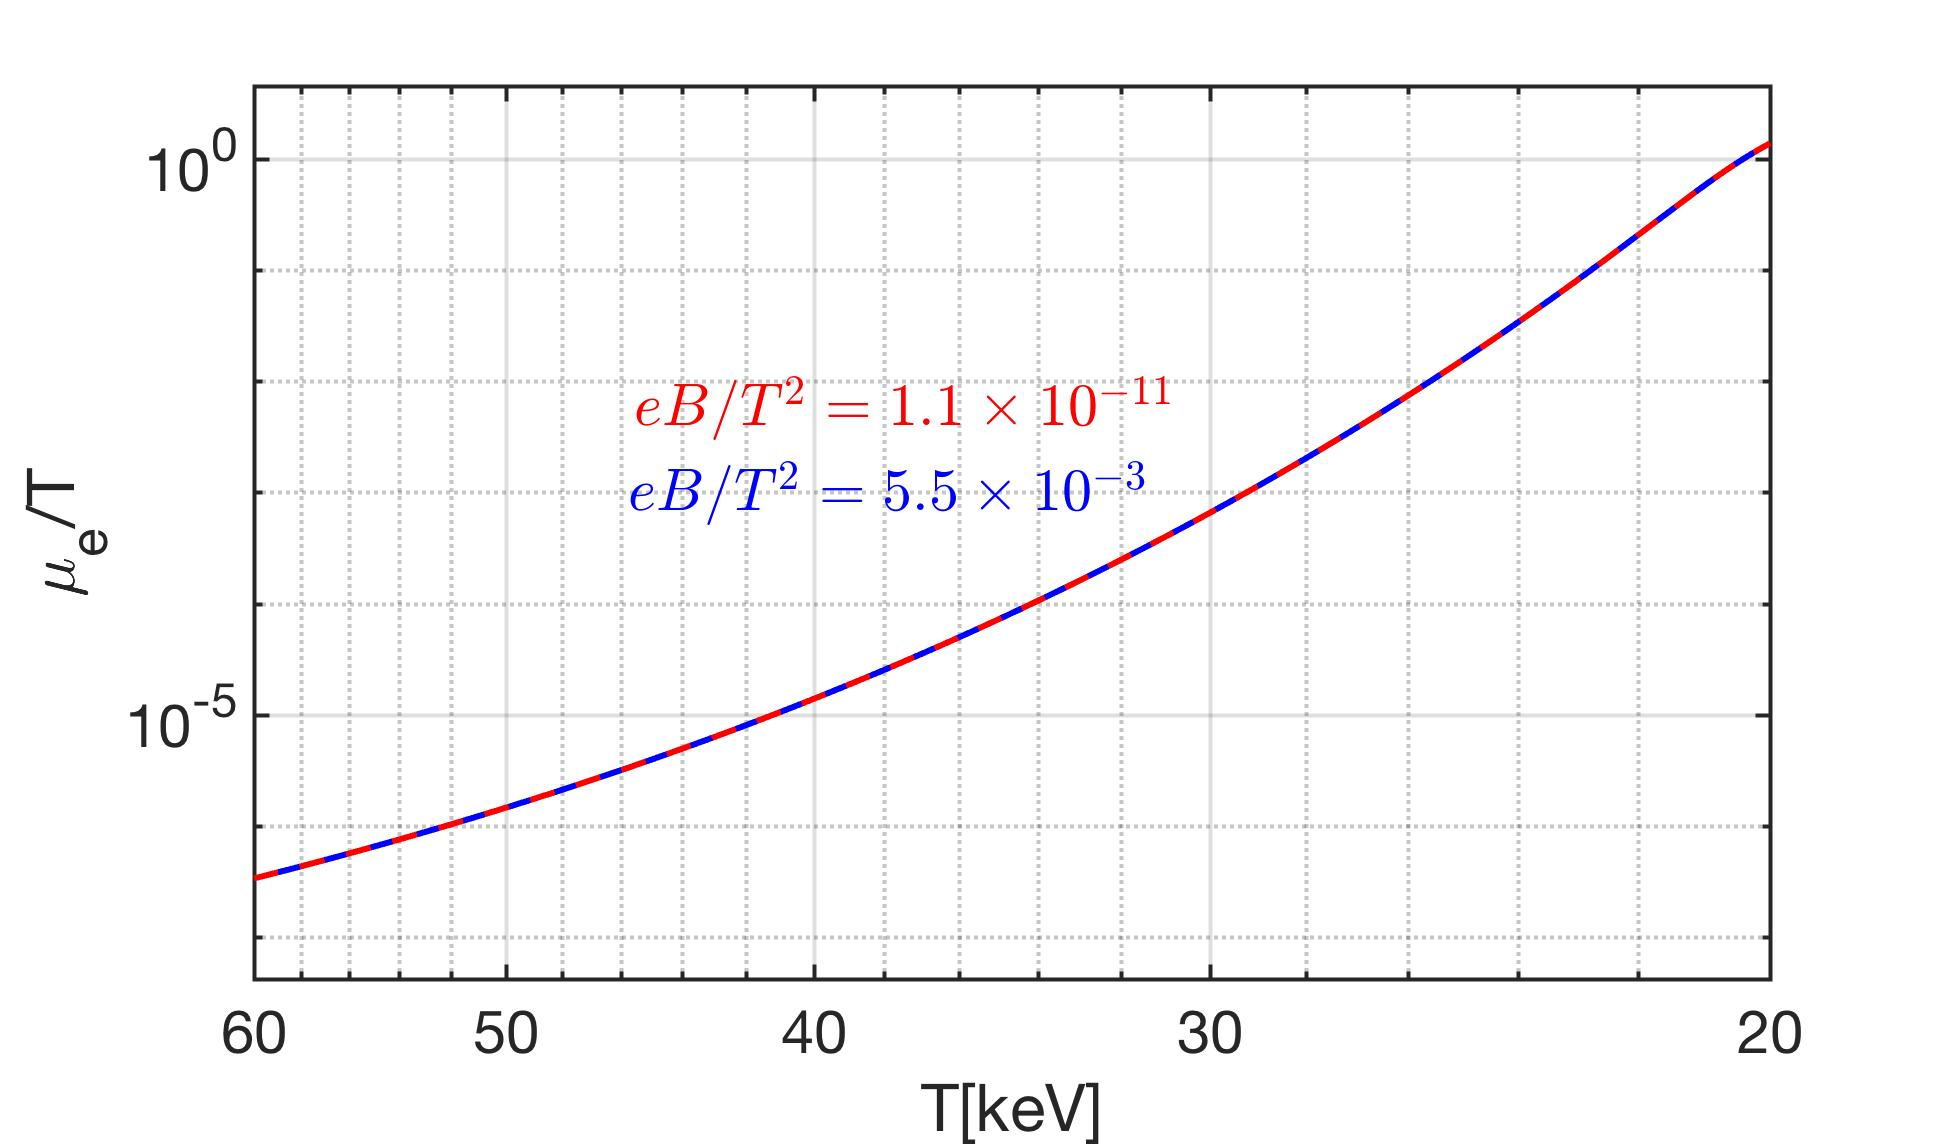
\includegraphics[width=0.75\linewidth]{./plots/ChemicalPotential_case1.jpg}
\caption{The chemical potential $\eta_{e}/T$ a function of temperature $20<T<60$keV.  It shows that the chemical potential is not sensitive to the magnetic field $b_0$.}
\label{chemical_fig} 
\end{figure}
%%%%%%%%%%%%%%%%%%%%%%%%%%%%%%%%%%%%%%%%%%%%%%%%%%%%%%%%%%%%%%%%%%
In {\rf{chemical_fig}}, we plot the  chemical potential as a function of temperature $T$. It shows that the chemical potential is not sensitive to the magnetic field because the small value of $b_0=10^{-3}\sim10^{-8}$ and can be neglected in \req{ChemicalPotential}. 

\subsection{Magnetization}
On the other hand, giving the partition function \req{lnZ} the magnetization can be obtained via the definition
\begin{align}
M=\frac{T}{V}\frac{\partial \ln\mathcal{Z}_{tot}}{\partial B}=\frac{T}{V}\left(\frac{\partial\tilde m_\pm}{\partial B}\right)\frac{\partial \ln\mathcal{Z}_{tot}}{\partial\tilde m_\pm}
\end{align}
Using the the dimensionless variables:
\begin{align}
x_\pm=\frac{\tilde m_\pm}{T},\qquad b_0=\frac{eB}{T^2}
\end{align}
then the magnetization can be written as
\begin{align}\label{Magnetization}
\left(\frac{M}{B}\right)=\frac{4\pi\alpha}{(2\pi)^2b_0}\left[2\cosh\left(\frac{\eta_{e}}{T}\right)\right]\left\{\left[1-\frac{(1\pm g/2)}{2}\left(1+\frac{b^2_0}{6x^2_\pm}\right)\right]x_\pm K_1(x_\pm)+\left[\frac{1}{3}-\frac{(1\pm g/2)}{2}\right]b_0K_0(x_\pm)\right\}.
\end{align}
Substituting the chemical potential \req{ChemicalPotential} into \req{Magnetization} we obtain
\begin{align}
\frac{M}{B}=\frac{8\pi\alpha}{(2\pi)^2b_0}&{\left(\left[1-\frac{(1\pm g/2)}{2}\left(1+\frac{b^2_0}{6x^2_\pm}\right)\right]x_\pm K_1(x_\pm)+\left[\frac{1}{3}-\frac{(1\pm g/2)}{2}\right]b_0K_0(x_\pm)\right)}\notag\\
&\qquad\times\sqrt{1+\left[\frac{{(2\pi)^2n_p}/{(2T^3)}}{x_\pm^2K_2(x_\pm)+b_0x_\pm K_1(x_\pm)+\frac{b^2_0}{6}K_0(x_\pm)}\right]^2}
\end{align}
In this case, given the magnetic field $B$ and chemical potential we can solve the magnetization $M$ as a function of temperature numerically.

%%%%%%%%%%%%%%%%%%%%%%%%%%%%%%%%%%%%%%%%%%%%%%%%%%%%%%%%%%%%%%%%%%
In our calculation we introduce an effective mass term which incorporates the ground state component of the Landau energy as follow
\begin{align}
x_\pm=\frac{\tilde{m}_\pm}{T}=\frac{1}{T}\sqrt{m^2_e+eB\left(1\pm\frac{g}{2}\right)}
\end{align}
Considering the case $g=2$ we have following two cases:
\begin{itemize}
  \item Case1: $\tilde m_+=\sqrt{m^2_e+2eB}$, and $x=\tilde m_+/T$. The magnetization is given by
  \begin{align}\label{Magnetization_001}
 \left(\frac{M}{B}\right)&=-\frac{8\pi\alpha}{(2\pi)^2}\left(\frac{b_0}{6x}K_1(x_\pm)+\frac{2}{3}K_0(x_\pm)\right)\sqrt{1+\left[\frac{{(2\pi)^2n_p}/{(2T^3)}}{\left[x_\pm^2K_2(x_\pm)+b_0x_\pm K_1(x_\pm)+\frac{b^2_0}{6}K_0(x_\pm)\right]}\right]^2}
   \end{align}
Substituting the magnetic field $b_0$ and proton density $n_p/T^3$  we can solve the magnetization and chemical potential numerically. In \rf{Case1_fig}, we plot the  magnetization $M/B$ as a function of temperature $T$. It shows for the case1 the magnetization is not sensitive to the magnetic field, this is because the small value of $b_0=10^{-3}\sim10^{-8}$ and can be neglected in \req{chemical_001} and \req{Magnetization_001}.
%%%%%%%%%%%%%%%%%%%%%%%%%%%%%%%%%%%%%%%%%%%%%%%%%%%%%%%%%%%%%%%%%%
\begin{figure}[t]
%\begin{center}
\centering
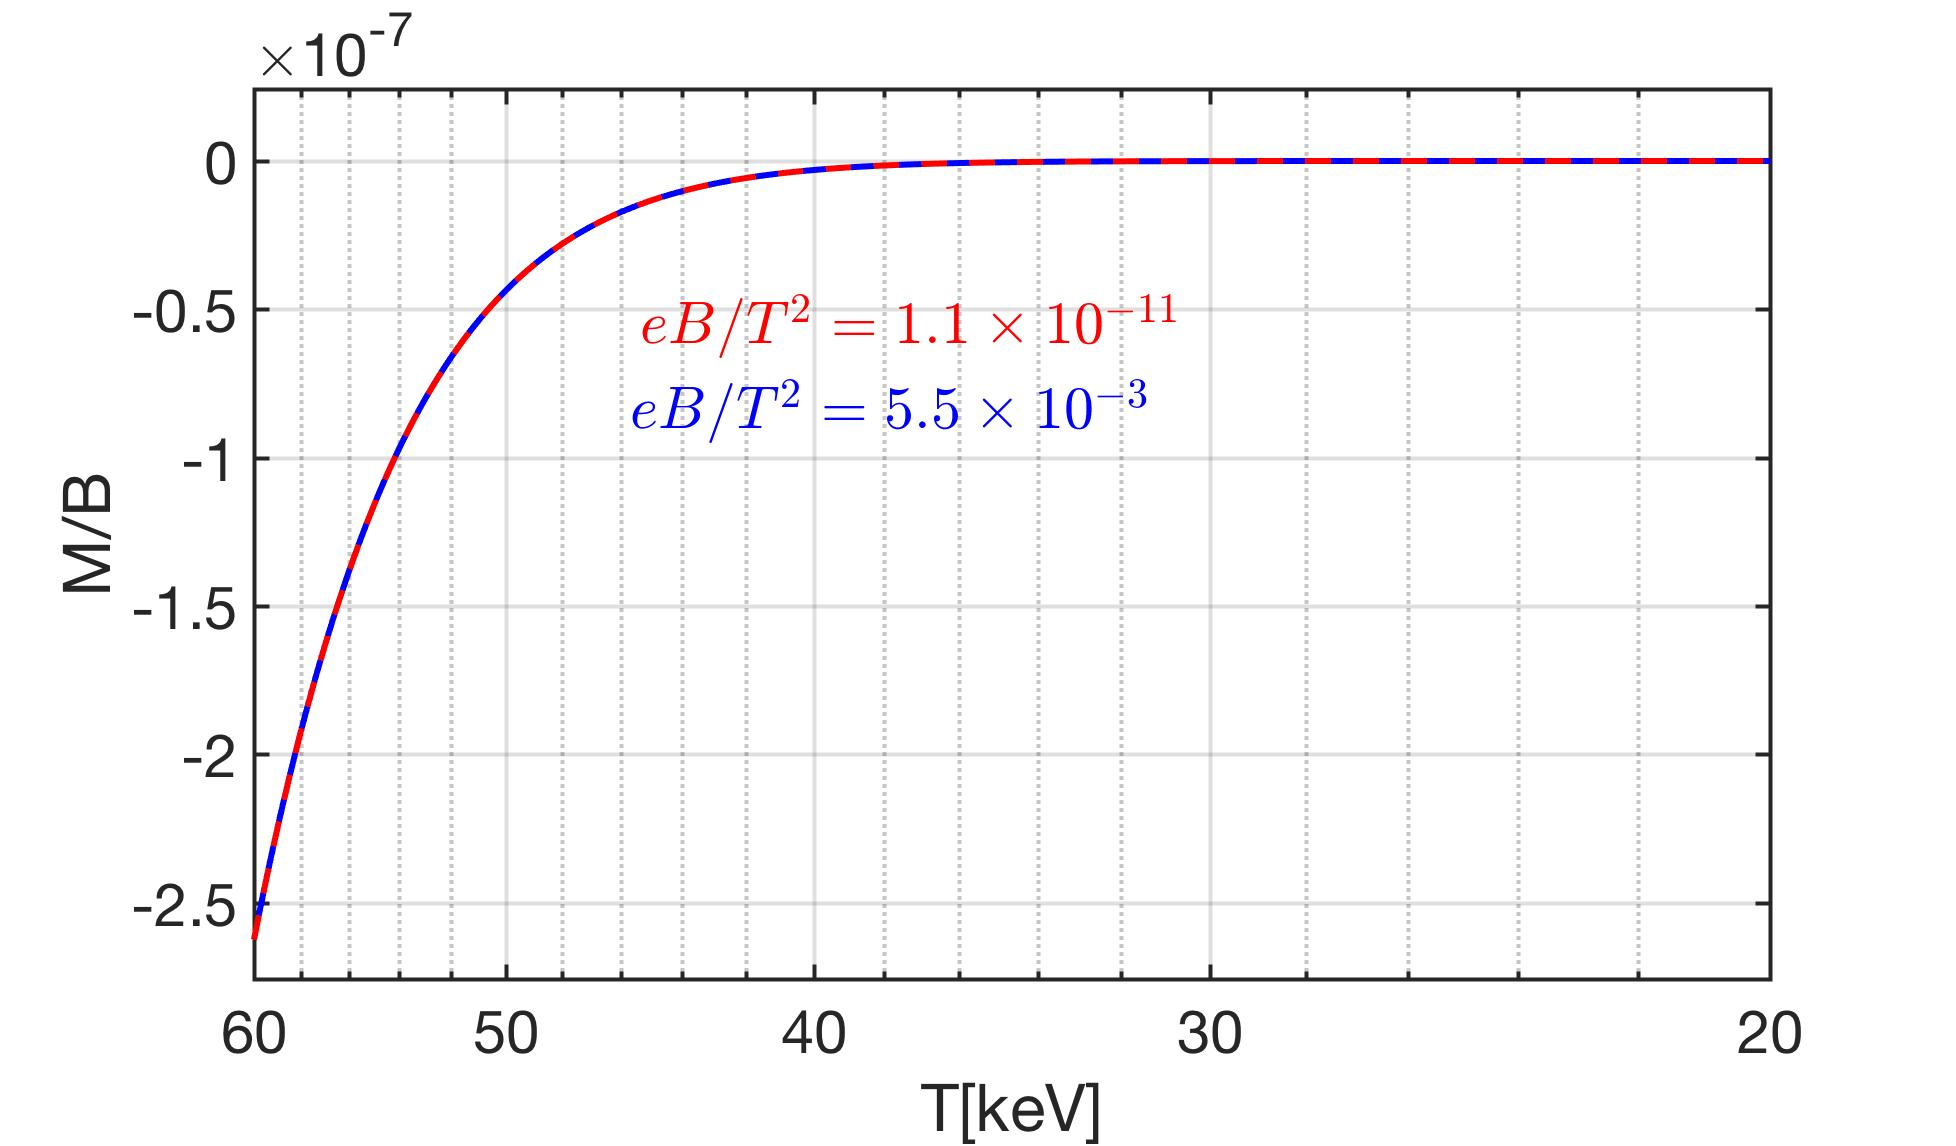
\includegraphics[width=0.75\linewidth]{./plots/Magnetization_case1.jpg}
\caption{The chemical potential $\eta_{e}/T$ (upper) and magnetization $M/B$ (lower) as a function of temperature $20<T<60$keV  for the case 1. The chemical potential and magnetization are not sensitive to the magnetic field, because the small value of $b_0=10^{-3}\sim10^{-8}$ can be neglected in \req{chemical_001} and \req{Magnetization_001}. }
\label{Case1_fig} 
\end{figure}
%%%%%%%%%%%%%%%%%%%%%%%%%%%%%%%%%%%%%%%%%%%%%%%%%%%%%%%%%%%%%%%%%%
\\
  \item Case 2: $\tilde m_-=m_e$ and $x=\tilde m_-/T$,then the magnetization of electron/ positron becomes
\begin{align}\label{Magnetization_002}
\left(\frac{M}{B}\right)&=\frac{8\pi\alpha}{(2\pi)^2}\left(\frac{1}{b_0}xK_1(x)+\frac{1}{3}K_0(x)\right)\sqrt{1+\left[\frac{{(2\pi)^2n_p}/{(2T^3)}}{\left[x^2K_2(x)+b_0x K_1(x)+\frac{b^2_0}{6}K_0(x)\right]}\right]^2}
\end{align}
Using the magnetic field $b_0$ and proton density $n_p/T^3$ we solve the magnetization  for case 2 numerically. In \rf{Case2_fig}, we plot the  magnetization $M/B$ as a function of temperature $T$. It shows that the magnetization depends on the magnetic field $b_0$ strongly. This is because for a small magnetic field $b_0$ the dominant term in \req{Magnetization_002} is $xK_1(x)/b_0$. For given $b_0$, the value of magnetization can be larger than the magnetic field, i.e. $M/B>1$  which shows the possibility that magnetic domains can be formed in the early universe.

%%%%%%%%%%%%%%%%%%%%%%%%%%%%%%%%%%%%%%%%%%%%%%%%%%%%%%%%%%%%%%%%%%
\begin{figure}[h]
%\begin{center}
\centering
%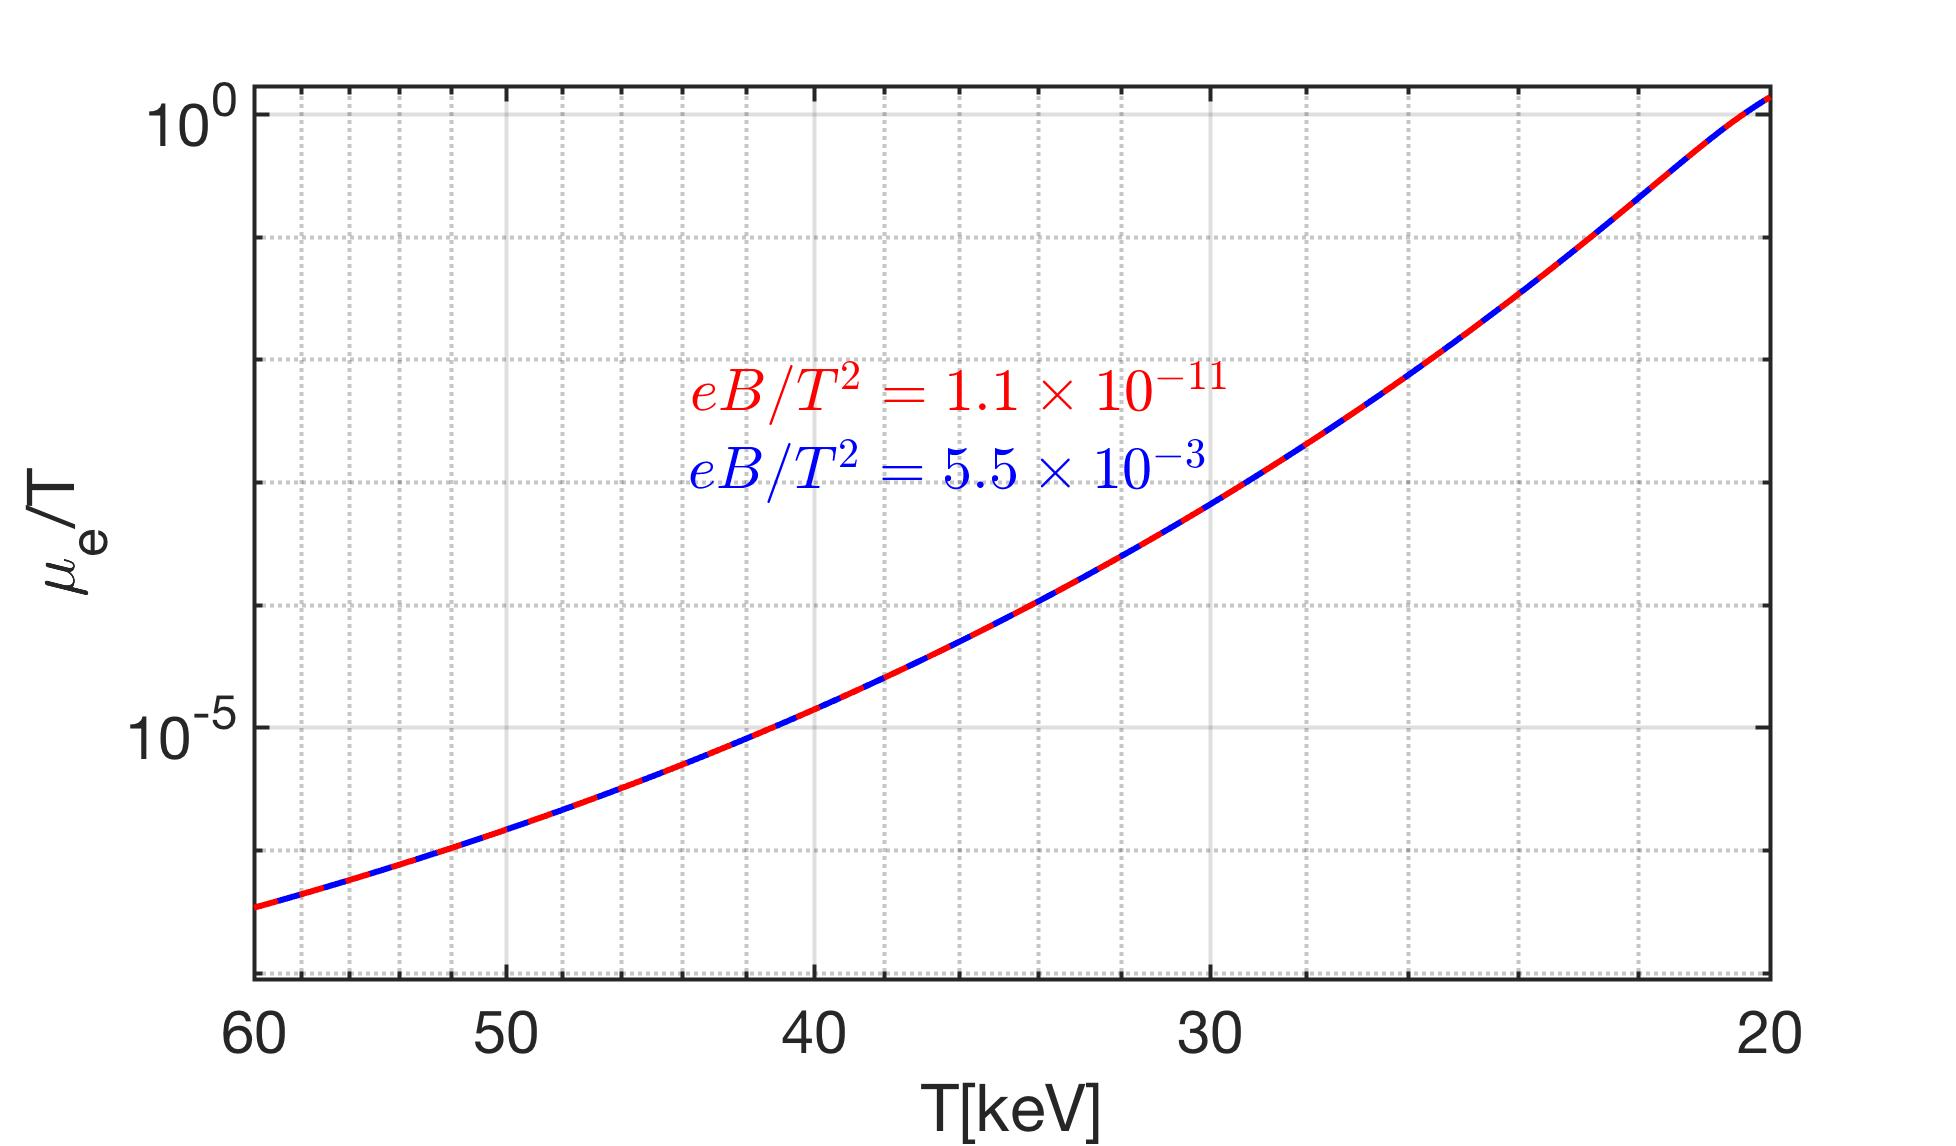
\includegraphics[width=0.75\linewidth]{./plots/ChemicalPotential_case2.jpg}
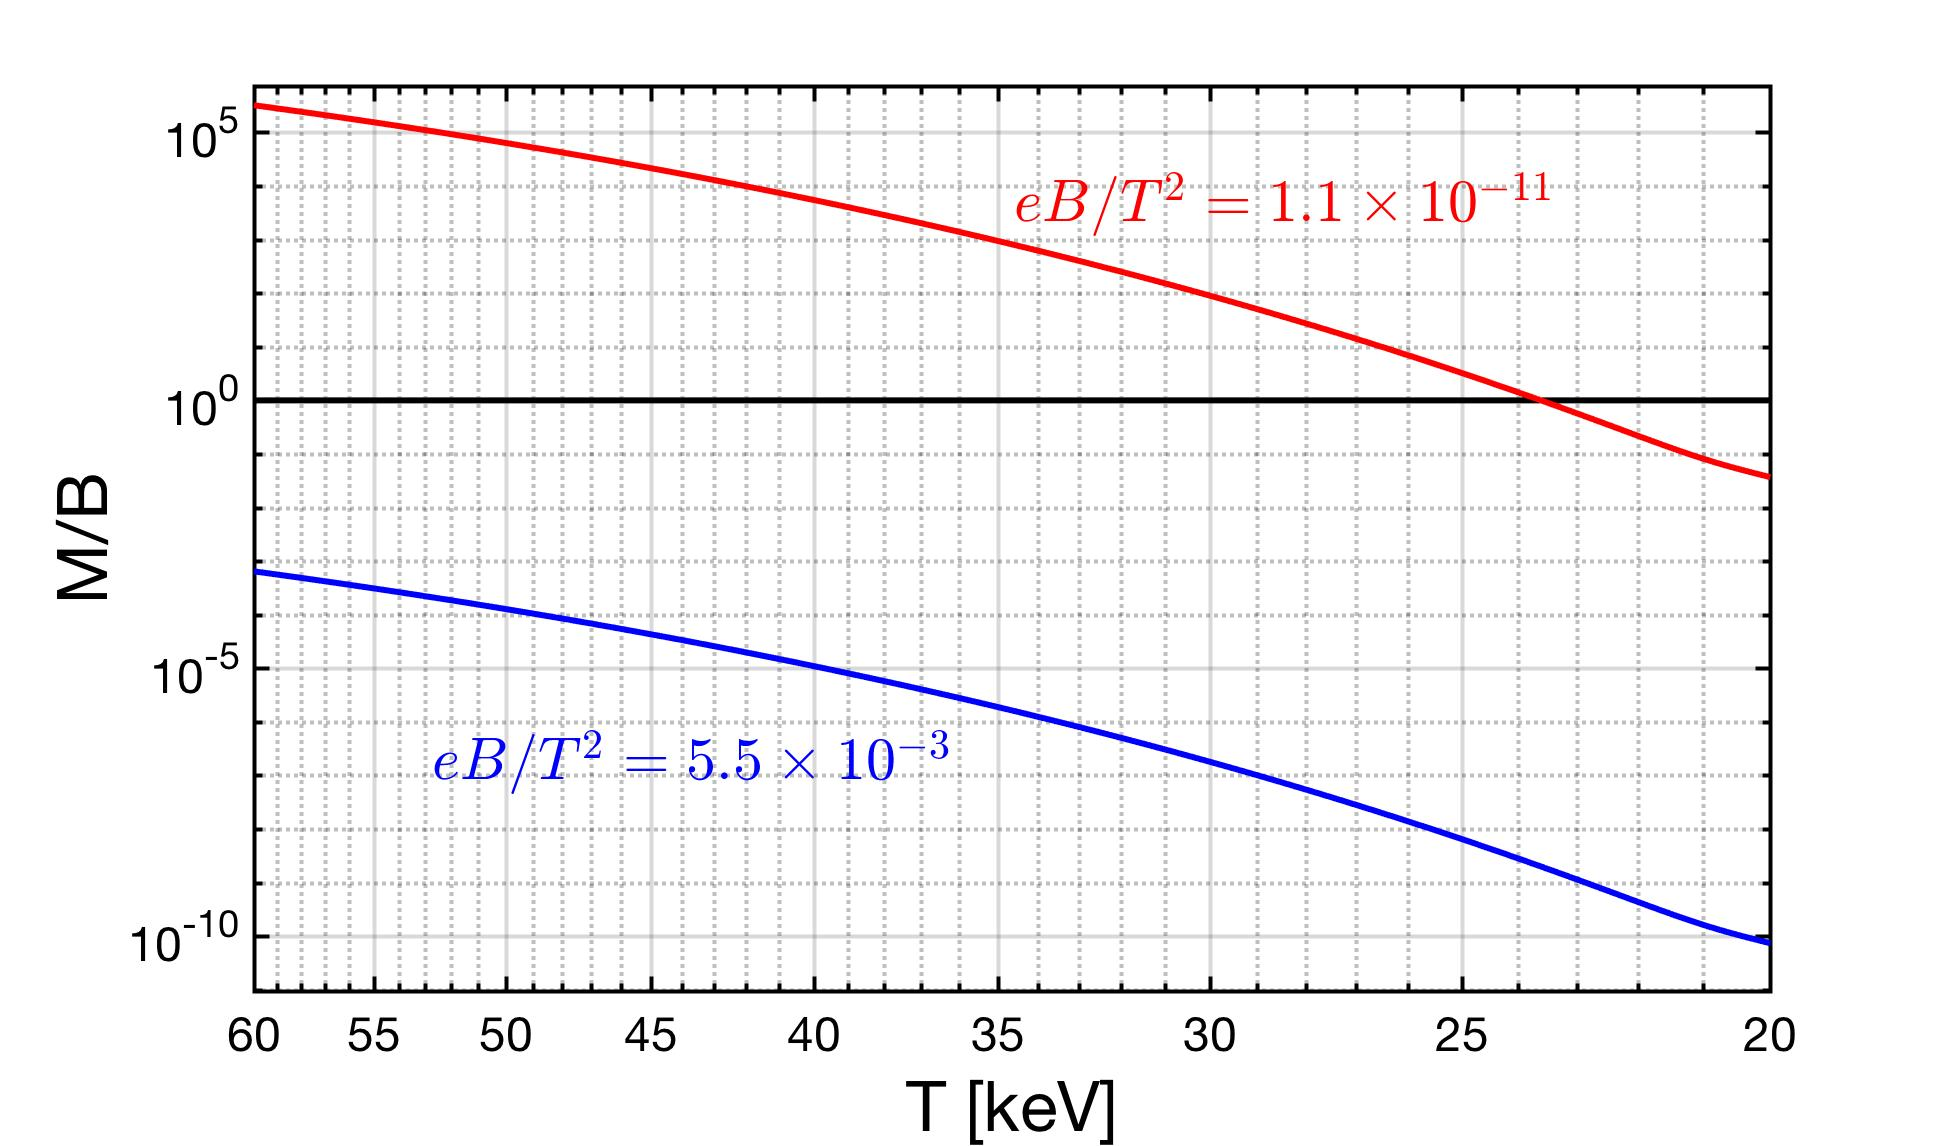
\includegraphics[width=0.75\linewidth]{./plots/Magnetization_case2.jpg}
\caption{The chemical potential $\eta_{e}/T$(upper) and magnetization $M/B$(lower) as a function of temperature $20<T<60$keV  for the case 2.  It shows that for giving $b_0$ we can find the temperature that $M/B>1$ in early universe.}
\label{Case2_fig} 
\end{figure}
%%%%%%%%%%%%%%%%%%%%%%%%%%%%%%%%%%%%%%%%%%%%%%%%%%%%%%%%%%%%%%%%%%

\end{itemize}
%%%%%%%%%%%%%%%%%%%%%%%%%%%%%%%%%%%%%%%%%%%%%%%%%%%%%%%%%%%%%%%%%%

\reftitle{References}
\begin{thebibliography}{99}

\bibitem{Fromerth:2012fe}
M.~J.~Fromerth, I.~Kuznetsova, L.~Labun, J.~Letessier and J.~Rafelski,
``From Quark-Gluon Universe to Neutrino Decoupling: 200 < T < 2MeV,''
Acta Phys. Polon. B \textbf{43}, no.12, 2261-2284 (2012)
doi:10.5506/APhysPolB.43.2261

\bibitem{Yang:2021bko}
C.~T.~Yang and J.~Rafelski,
``Cosmological strangeness abundance,''
Phys. Lett. B \textbf{827}, 136944 (2022)
doi:10.1016/j.physletb.2022.136944

\bibitem{Birrell:2012gg} 
J.~Birrell, Cheng~Tao~Yang, P.~Chen and J.~Rafelski,
\lq\lq Relic neutrinos: Physically consistent treatment of effective number of neutrinos and neutrino mass,\rq\rq
Phys.\ Rev.\ D {\bf 89}, 023008 (2014)
doi:10.1103/PhysRevD.89.023008
[arXiv:1212.6943 [astro-ph.CO]].

\bibitem{Chris:2023abc}
Christopher Grayson, C.~T.~Yang and J.~Rafelski,
``Electron-Positron Plasma in BBN epoch,'' (to be published).

\bibitem{Pitrou:2018cgg} 
C.~Pitrou, A.~Coc, J.~P.~Uzan and E.~Vangioni,
\lq\lq Precision big bang nucleosynthesis with improved Helium-4 predictions,\rq\rq\ 
arXiv:1801.08023 [astro-ph.CO], Phys. Rep. {\it in press} (2018)


\bibitem{Wang:2010px} 
B.~Wang, C.~A.~Bertulani and A.~B.~Balantekin,
\lq\lq Electron screening and its effects on Big-Bang nucleosynthesis, \rq\rq
Phys.\ Rev.\ C {\bf 83}, 018801 (2011)
doi:10.1103/PhysRevC.83.018801
[arXiv:1010.1565 [astro-ph.CO]].

\bibitem{Mangano:2005cc} 
G.~Mangano, G.~Miele, S.~Pastor, T.~Pinto, O.~Pisanti and P.~D.~Serpico,
\lq\lq Relic neutrino decoupling including flavor oscillations,\rq\rq\
Nucl.\ Phys.\ B {\bf 729}, 221 (2005)
doi:10.1016/j.nuclphysb.2005.09.041
[hep-ph/0506164].

\bibitem{Birrell:2014uka} 
 J.~Birrell, Cheng~Tao~Yang and J.~Rafelski,
\lq\lq Relic Neutrino Freeze-out: Dependence on Natural Constants,\rq\rq\
 Nucl.\ Phys.\ B {\bf 890}, 481 (2014)
 doi:10.1016/j.nuclphysb.2014.11.020
 [arXiv:1406.1759 [nucl-th]].


\bibitem{ParticleDataGroup:2022pth}
R.~L.~Workman \textit{et al.} [Particle Data Group],
``Review of Particle Physics,''
PTEP \textbf{2022}, 083C01 (2022)
doi:10.1093/ptep/ptac097

\bibitem{Kolb:1990vq} 
E.~W.~Kolb and M.~S.~Turner,
\emph{The Early Universe},
547 pp, Front.\ Phys.\ {\bf 69}, 1 (1990),
ISBN: 0201626748, 9780201626742


 

%\bibitem{Aksenov:2007}
%A. G. Aksenov, R. Ruffini, and G. V. Vereshchagin
%``Thermalization of Nonequilibrium Electron-Positron-Photon Plasmas,''
%Phys.\ Rev.\ Lett.\ \textbf{99}, 125003 (2007) 
%doi: 10.1103/PhysRevLett.99.125003

%\bibitem{Aksenov:2010}
%A. G. Aksenov, R. Ruffini, and G. V. Vereshchagin
%``Pair plasma relaxation time scales''
%Phys.\ Rev.\ E \textbf{81}, 046401 (2010)
%doi: 10.1103/PhysRevE.81.046401
\end{thebibliography}

%%%%%%%%%%%%%%%%%%%%%%%%%%%%%%%%%%%%%%%%%%
\end{document}
